% !TeX spellcheck = en_US
\documentclass[preprint,authoryear]{elsarticle}
% sudo apt-get install -y texlive-publishers

\usepackage[left]{lineno}
\usepackage[utf8]{inputenc}
\usepackage[T1]{fontenc}
\usepackage{lmodern}
\usepackage{multirow}

\usepackage{lineno,hyperref}
\modulolinenumbers[5]

%\usepackage{hyphenat}
\usepackage[none]{hyphenat}

\usepackage{url}
\usepackage{booktabs}

\usepackage{mathtools}
\usepackage{amssymb}
\usepackage{amsthm}

\usepackage{caption}
\captionsetup{labelfont=bf}
\captionsetup{skip=0pt} % vertical distance from the table or figure


\usepackage{algorithm} % sudo apt-get install -y texlive-science

\usepackage[noend]{algpseudocode}

\usepackage[margin=0.9in]{geometry}

\usepackage[normalem]{ulem}
\usepackage{xcolor}

\newcommand{\Comentar}[1]{\State {\cmmt{#1}}}
\newcommand{\Break}{\State \bf {break}}
\renewcommand{\Return}{\State \bf {return}~}
\renewcommand{\algorithmicensure}{\bf {Parameters:}}

\renewcommand\algorithmicthen{}
\renewcommand\algorithmicdo{}


\algblock{ForEach}{EndFor}
\algblock{ForDownTo}{EndFor}
\algblock{ForTo}{EndFor}

\newcommand{\Block}[1]{\State #1 \{}
\newcommand{\EndBlock}{\State \}}

%----- begin celio
\usepackage{scrextend}
\newcommand{\boldm}[1] {\mathversion{bold}#1\mathversion{normal}}
\newcommand{\round}[1]{\ensuremath{\lfloor#1\rceil}}
\usepackage{setspace}
\usepackage{array}
\usepackage{color, colortbl}
\definecolor{Gray}{gray}{0.9}

\newcommand{\specialcell}[2][c]{%
	\begin{tabular}[#1]{@{}c@{}}#2\end{tabular}}

\usepackage{tikz}
\usetikzlibrary{calc}
\usetikzlibrary{positioning}

\usepackage{pgfplots}

\pgfplotsset{
	compat=1.9,
	myplotstyle/.style={
		legend cell align=left,
		every axis plot/.append style={thick},
		legend style={font=\small,draw=none},
		enlargelimits=0.2,
		legend pos=south east,
		y tick label style={ /pgf/number format/.cd, fixed, fixed zerofill, precision=3, /tikz/.cd, },
		x tick label style={ /pgf/number format/.cd, fixed, fixed zerofill, precision=1, /tikz/.cd, },
		grid=major,		
	},
}

\usepackage{float}% http://ctan.org/pkg/float


%----- end celio

\journal{Computers \& Operations Research}


\begin{document}


\begin{frontmatter}

\title{Parallel air palletization and tour planning for simultaneous pickup and delivery}

\author{A.C.P.~Mesquita}
\ead{celio@ita.br}

\author{C.A.A.~Sanches\corref{cor1}}
\ead{alonso@ita.br}
\cortext[cor1]{Corresponding author.}

\address {Instituto Tecnol\'{o}gico de Aeron\'{a}utica - DCTA/ITA/IEC\\
Pra\c{c}a Mal. Eduardo Gomes, 50\\
S\~{a}o Jos\'{e} dos Campos - SP - 12.228-900 - Brazil}


\begin{abstract}

Transport aviation faces risks of cargo imbalance in the set of circumstances of aerial pickup and shipment of goods in a distribution system given the urgency required for loading for fast takeoff and mission accomplishment, notably in moments of crisis, public emergency, client contract short turnaround times, or any external forces for instant takeoff. Additionally, there is no computer support to aid load and trip programmers with the massive transportation demands in each location.

Other dangers are made possible as a result, including poor delivery, excessive fuel consumption, and longer turnaround times than necessary.

We developed an efficient solution by means of computer parallelism to the problem involving scheduling the loading and routing of an airplane in a tour of simultaneous pickup and delivery at intermediate hubs while taking into account a utility score, weight and balance rules, and fuel usage.

This hard problem, named {\it Air Cargo Load Planning with Routing, Pickup, and Delivery Problem} considers using standardized pallets in fixed positions, obeying the center of gravity constraints, delivering each item to its destination, and minimizing fuel consumption costs.

We also contributed by carrying out multiple experiments with the well-known Ant Colony Optimization on synthetic data based on real data from the {\it Brazilian Air Force}\/ transportation history and a new procedure to minimize the distance from the next node destined pallet to the ramp door.

We also created a process-based parallel computing heuristic that quickly finds good solutions for a wide range of problem sizes, an essential contribution as { \color{red} it was the unique method that managed to solve all testing scenarios.}

\end{abstract}

\begin{keyword}
Air Cargo \sep Air Palletization \sep Weight and Balance \sep Pickup and Delivery \sep Vehicle Routing \sep Parallel computing
\end{keyword}

\end{frontmatter}

\label{sec1}
\section{Introduction}


Air cargo transport involves several sub-problems that are difficult to solve. Recently, \cite{MesquitaSanches2023} modeled and solved the {\it Air Cargo Load Planning with Routing, Pickup and Delivery} (ACLP+RPDP) composed by four sub-problems: {\it Build-up Scheduling Problem}, {\it Air Palletization Problem} (APP), {\it Weight and Balance Problem} (WBP), and a special case of the {\it Traveling Salesman Problem}, similar to the proposed by \cite{kaspi2019}, where the profit per unit time is defined as the profit gained after completing the tour divided by the total time (cost in our case) required to complete the tour.

However, there are still other important challenges in air cargo transport that go beyond the definition of the ACLP+RPDP, especially with regard to algorithms performance and the easiness of loading operations at each destination.

Considering air cargo transport, Table \ref{tab:sa} lists the main works in the literature and the corresponding sub-problems addressed. We also indicate whether the dimensions of the items were taken into account ({\bf 3D} or {\bf 2D}) and which solution method was used: heuristics ({\bf Heu}), integers ({\bf Int}), or linear programming ({\bf Lin}).

\begin{table}[H]
	\centering
	\caption{Air cargo transport: literature, problems and features}  \label{tab:sa}
	\scriptsize
	\renewcommand{\arraystretch}{1.1} % alturas das linhas \specialcell{{\bf Parallel}\\{\bf heuristics}}
	\begin{tabular}{r|cc|cc|cc|ccc|c}
		\toprule
		                            & {\bf APP}  & {\bf WBP}  &  {\bf SPDP}   &{\bf TSP}   & {\bf 2D}  & {\bf 3D}  & {\bf Heu}  & {\bf Int}  & {\bf Lin} & \specialcell{{\bf Parallel}\\{\bf heuristics}}\\
		\midrule
		\cite{LarsenMikkelsen1979}  & $.$        & $\bigstar$ & $.$          & $.$        & $.$       & $.$       & $\bigstar$ & $.$        &  $.$&  $.$ \\
		\cite{Brosh1981}  & $.$ & $\bigstar$  & $.$   & $.$ & $.$ & $.$   & $.$  & $.$  &  $\bigstar$&  $.$ \\
		\cite{Kevin1992}  & $.$ & $\bigstar$  & $.$ & $.$ & $.$ &$.$   & $.$  & $\bigstar$  &  $.$ &  $.$\\
		\cite{Heidelberg1998}  & $.$ & $\bigstar$  & $.$ & $.$ & $\bigstar$ &$.$   & $\bigstar$  & $.$  &  $.$&  $.$ \\
		\cite{MongeauBes2003}    & $\bigstar$ & $\bigstar$   & $.$ & $.$ & $.$ & $.$   & $.$  & $\bigstar$  &  $.$ &  $.$\\
		\cite{fok2004optimizing} & $.$ & $\bigstar$   & $.$ & $.$ & $.$ & $.$   & $.$  & $\bigstar$  &  $.$&  $.$ \\	
		\cite{Chan2006}  & $\bigstar$ & $.$    & $.$ & $.$ & $.$ & $\bigstar$  & $\bigstar$  & $.$  &  $.$&  $.$ \\
		\cite{KaluznyBohdanL2009Oalb}  & $.$ & $\bigstar$  & $.$  & $.$ & $\bigstar$ &$.$  & $.$  & $\bigstar$  &  $.$&  $.$ \\
		\cite{Verstichel2011}   & $.$ & $\bigstar$    & $.$ & $.$ & $.$ & $.$   & $.$  & $\bigstar$  &  $.$&  $.$ \\
		\cite{MesquitaCunha2011}   & $.$ & $.$    & $\bigstar$ & $.$ & $.$ & $.$   & $\bigstar$  & $.$  &  $.$ &  $.$\\		
		\cite{Limbourg2012} & $.$ & $\bigstar$  & $.$ & $.$ & $.$ & $.$   & $.$  & $\bigstar$  &  $.$&  $.$ \\
		
		\cite{kaspi2019} & $.$ & $.$  & $.$ & $\bigstar$ & $.$ & $.$   & $\bigstar$  & $.$  &  $.$&  $.$ \\
		
		\cite{RoesenerHall2014}  & $\bigstar$ & $\bigstar$  & $.$  & $.$ & $.$ & $\bigstar$   & $.$  & $\bigstar$  &  $.$&  $.$ \\
		\cite{Vancroonemburg2014}  & $\bigstar$ & $\bigstar$   & $.$ & $.$ & $.$ & $.$   & $.$  & $\bigstar$  &  $.$&  $.$ \\
		\cite{LurkinSchyns2015} & $.$ & $\bigstar$  & $\bigstar$ & $.$  & $.$ & $.$   & $.$  & $\bigstar$  &  $.$&  $.$ \\
		\cite{RoesenerBarnes2016}  & $.$ & $\bigstar$   & $.$ & $.$ & $.$ & $.$   & $\bigstar$  & $.$  &  $.$&  $.$ \\
		\cite{PaquaySchynsLimbourg2016,PaquayLimbourgSchynsOliveira2018}  & $\bigstar$ & $\bigstar$ & $.$ & $.$ & $.$ & $\bigstar$ & $\bigstar$  & $\bigstar$ & $.$&  $.$ \\
		\cite{YangLiuGao2018} & $.$ & $\bigstar$  & $.$  & $.$ & $\bigstar$  & $.$ & $\bigstar$ & $.$  & $.$&  $.$ \\
		\cite{wong2020} & $\bigstar$  & $\bigstar$  & $.$  & $.$   & $.$  & $.$ & $.$ & $\bigstar$  & $.$&  $.$  \\
		\cite{eugene2021} & $\bigstar$ & $\bigstar$ & $.$  & $.$   & $.$ & $.$ & $.$ & $\bigstar$  & $.$&  $.$  \\
		\cite{zhao2021} & $.$ & $\bigstar$ & $.$  & $.$  & $.$ & $.$ & $.$  & $\bigstar$ &  $.$&  $.$ \\
		
		\cite{MesquitaSanches2023}   & $\bigstar$ & $\bigstar$  & $\bigstar$& $\bigstar$ & $.$ & $.$ & $\bigstar$ & $\bigstar$   &  $.$&  $.$  \\
		
		{\bf This work}   & $\bigstar$ & $\bigstar$  & $\bigstar$& $\bigstar$ & $.$ & $.$ & $\bigstar$ & $\bigstar$   &  $.$&  $\bigstar$  \\
		\bottomrule 
	\end{tabular}
	\normalsize 
\end{table}

As can be seen, so far \cite{LurkinSchyns2015} is the only work that simultaneously addresses an air cargo (WBP) and a flight itinerary (PDP) sub-problem. Although it is innovative, strong simplifications were imposed by the authors: in relation to loading, APP was ignored; with regard to routing, it is assumed a pre-defined flight plan restricted to two legs. It is important to note that these authors consider an aircraft with two doors, and the minimization of loading and unloading costs at the intermediate node was modelled through a container sequencing problem. Referring directly to this work, \cite[p. 409]{BrandtStefan2019} comment: {\it However, not even these sub-problems are acceptably solved for real-world problem sizes or the models omit some practically relevant constraints}. 

There are real situations that are much more complex. In this work, we consider a practical case in Brazil, which is the largest economy in Latin America. Due to its dimensions, this country has the largest air market on the continent with $2,499$\/ registered airports, of which $1,911$\/ are private and $588$\/ are public. Although it is an immense distribution network, airlift missions consider 3 to 5 nodes per flight plan. Throughout this work, we address routes with up to 7 nodes, as can be seen in Table \ref{tab:costs} and Figure \ref{fig:nodes}.


\begin{table}[H]
	
	\begin{minipage}{0.05\linewidth}
		
	\end{minipage}\hfill % these two lines must be close to each other
	\begin{minipage}{0.45\linewidth}
		
		\caption{Brazilian airports distances ($km$)}  \label{tab:costs}
		\centering
		
		\footnotesize
		
		\newcolumntype{Y}{>{\centering\arraybackslash}p{0.09\textwidth}}
		\newcolumntype{X}{>{\centering}p{0.09\textwidth}}
		
		\begin{tabular}{X X X X X X X Y}
			\toprule
			Node & $l_0$ & $l_1$ & $l_2$ & $l_3$ & $l_4$ & $l_5$ & $l_6$ \\
			IATA*   & GRU   & GIG   & SSA   & CNF   & CWB   & BSB   & REC \\	
			\midrule	
			GRU     & 0	    &343	&1,439   &504    &358    &866    &2,114\\
			GIG	    & 343	&0	    &1,218   &371    &677    &935    &1,876\\
			SSA	    & 1,439	&1,218	&0	    &938    &1,788   &1,062   &676\\
			CNF	    & 504	&371	&938	&0	    &851    &606    &1,613\\
			CWB	    & 358	&677	&1,788	&851	&0	    &1,084   &2,462\\
			BSB	    & 866	&935	&1,062	&606	&1,084	&0	    &1,658\\
			REC	    & 2,114	&1,876	&676	&1,613	&2,462	&1,658	&0\\
			\bottomrule
			\multicolumn{8}{c}{*International Air Transport Association}\\
			\multicolumn{8}{c}{\small\textsuperscript{Source: www.airportdistancecalculator.com}}\\
		\end{tabular}
		\normalsize
		
	\end{minipage}\hfill % these two lines must be close to each other
	\begin{minipage}{0.50\linewidth}
		\centering
		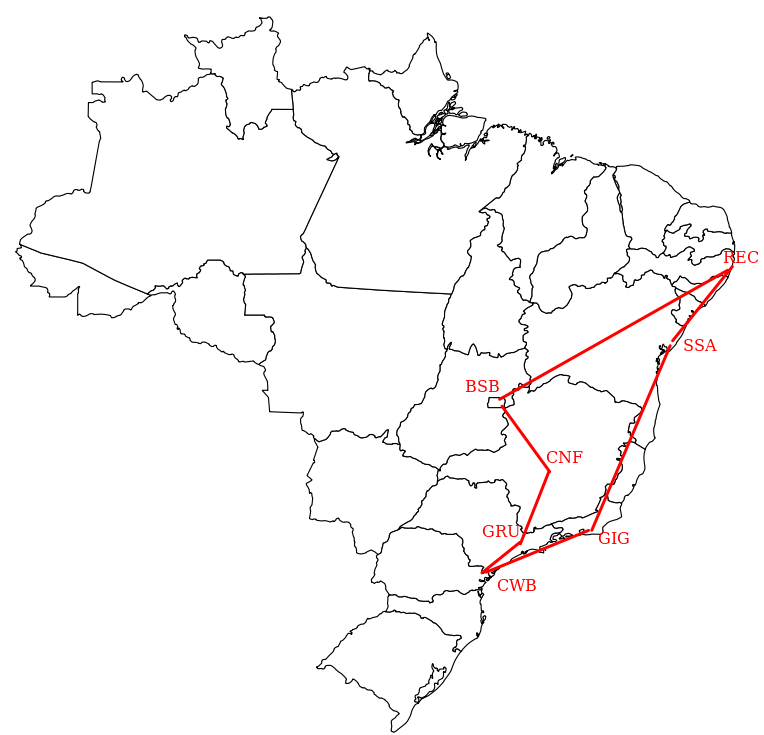
\includegraphics[scale=0.25]{Images/nodes.png}
		\captionof{figure}{A route between Brazilian airports}
		\label{fig:nodes}		
	\end{minipage}
\end{table}


In the {\it Brazilian Air Force}\/ missions, hundreds of items can be carried at each node, where the objectives are to prioritize the transport of the most important items and minimize the cost of fuel along the route. As standardized pallets are used with predefined positions on the aircraft, it is possible to carry out loading and unloading at each node in around two hours. However, there is no technological assistance that guarantees the achievement of these objectives.

\cite{MesquitaSanches2023} proposed a method that attends these objectives: a pallet building and arrangement plan with a routing option that maximizes the benefit-cost ratio for the smooth execution of pickup and delivery transport missions. They develop a heuristic that can be executed on a simple handheld computer (like a laptop or a tablet) and that provides a solution quickly enough to keep this cargo handling time under an hour. This work seeks to improve their results in terms of quality and performance by the use of computer parallelism and by minimizing the distance between the next node destined pallets and the cargo door.

These improvements in their heuristics are meant to reduce the stress that transport planners are subjected to, because they have to deal with a lot of information in planning the aircraft route, assembling the pallets, and picking up and delivering at each node. To the best of our knowledge, that is the first time that an air cargo transport problem that simultaneously involves APP, WBP, PDP and TSP has been addressed, and the first time ACLP+RPDP is solved with computer parallelism.

This article is organized into six more sections. In Section \ref{sec2}, we give a brief review of the literature. In Section \ref{sec3}, we present the problem context and assumptions and, in Section \ref{sec4}, the mathematical model and how we dealt with its issues. In Section \ref{sec5}, we describe the elaborate algorithms, whose results are presented in Section \ref{sec6}. Finally, our conclusions are in Section \ref{sec7}.


\section{Related literature}
\label{sec2}

In this section, we briefly describe the characteristics of the main works related to air cargo transport, following the chronological order of Table \ref{tab:sa}.

\cite{LarsenMikkelsen1979} developed an interactive procedure for loading 14 types of Boeing 747 into a two-leg flight plan. Seven types of items were considered to be allocated in 17 to 42 positions. With non-linear programming and heuristics, they present a solution that minimizes positioning changes in the intermediate node, optimizing the load balancing in the aircraft.

\cite{Brosh1981} addressed the problem of planning the allocation of cargo on an aircraft. Considering volume, weight and structural constraints, the author finds the optimal load layout through a fractional programming problem.

\cite{Kevin1992} developed a multi-criteria optimization approach to load the {\it C-130} aircraft of the {\it Canadian Air Force}. Based on integer programming, this model provides timely planning and improves airlift support for combat operations, solving WBP with pallets in fixed positions, and considering 20 different items.

\cite{Heidelberg1998} developed a heuristic for 2D packing in air loading, comparing it with methods for solving the {\it Bin Packing Problem}. Authors conclude that the classical algorithms are inadequate in this context, because they ignore the aircraft balancing constraints.

\cite{MongeauBes2003} presented a method based on linear integer programming to solve the problem of choosing and positioning containers on the {\it Airbus 340-300}. Safety and stability constraints were considered, with the objective of minimizing fuel consumption.

\cite{fok2004optimizing} developed a web-based application to make efficient use of space and load balancing for an air cargo company. Based on an analysis of historical data, an operational load planning with mathematical optimization is obtained. This container load planning is usually done roughly 2 hours before departure, when all cargo details are in place.

\cite{Chan2006} carried out a case study with heterogeneous pallets. In order to minimise the total cost of shipping, they developed a 3D packing heuristic, with a loading plan for each pallet. Although the authors do not consider load balancing or positioning of pallets in the cargo hold, this method is relevant in commercial and industrial applications, where cargo items tend to be less dense.

\cite{KaluznyBohdanL2009Oalb} developed a mixed integer linear programming model to arrange a set of items in a military context that optimizes the load balance.

\cite{Verstichel2011} solved WBP by selecting the most profitable subset of containers to be loaded onto an aircraft using mixed-integer programming. Experimental results on real-life data showed significant improvements compared to those obtained manually by an experienced planner.

\cite{MesquitaCunha2011} presented a heuristic for a real problem of the {\it Brazilian Air Force}, which consists of defining transport routes with simultaneous collection and delivery from a central distribution terminal.

\cite{Limbourg2012} developed a mixed-integer program for optimally rearranging a set of pallets into a compartmentalized cargo aircraft, specifically the {\it Boeing 747}.

\cite{kaspi2019} define and solve a new extension of the TSP to maximize the financial contribution per invested time and present an optimal iterative solution procedure for the problem which converges after a limited number of iterations.

\cite{RoesenerHall2014} solved APP and WBP as an integer programming problem, which also allows items to be loaded into pallets according to a specific orientation (e.g., this side up).

\cite{Vancroonemburg2014} presented a mixed integer linear programming model that selects the most profitable pallets, satisfying safety and load balancing constraints on the {\it Boeing 747-400}. Using a solver, authors solved real problems in less than an hour.

As already mentioned, \cite{LurkinSchyns2015} was the first work that simultaneously modeled WBP and SPDP in air cargo transport. The authors demonstrated that this problem is NP-hard and performed some experiments with real data, noting that their model offers better results than those obtained manually.

\cite{RoesenerBarnes2016} proposed a heuristic to solve the {\it Dynamic Airlift Loading Problem} (DALP). Given a set of palletized cargo items that require transport between two nodes in a time frame, the objective of this problem is to select an efficient subset of aircraft, partition the pallets into aircraft loads and assign them to allowable positions on those aircraft.

\cite{PaquaySchynsLimbourg2016} presented a mathematical modeling to optimize the loading of heterogeneous 3D boxes on pallets with a truncated parallelepipeds format. Its objective is to maximise the volume used in containers, considering load balancing constraints, the presence of fragile items and the possibility of rotating these boxes. \cite{PaquayLimbourgSchynsOliveira2018} developed some heuristics to solve this problem.

\cite{YangLiuGao2018} modelled the air transport problem as a 2D packing problem, and presented a heuristic for its optimization in several aircraft, considering load balancing in order to minimise fuel consumption.

\cite{wong2020}A developed a mathematical model and a tool based on mixed integer programming for optimizing cargo in aircraft with different pallet configurations. Balance constraints and the presence of dangerous items were considered. \cite{eugene2021} integrated this tool to a digital simulation model, with a visualization and validation system, based on sensors that alert about load deviations.

\cite{zhao2021} proposed a new modelling for WBP based on mixed integer programming. Instead of focusing on the center of gravity (CG) deviation, the authors consider the original CG envelope of the aircraft, with a linearization method for its non-linear constraints.

\cite{MesquitaSanches2023} contributed with a complex model and elaborate heuristics for the ACLP-RPDP that simultaneously solve 4 intractable sub-problems: APP, WBP, SPDP and TSP. They also compare the performances of four well known heuristics: {\it Ant Colony Optimization}, the {\it Noising Method Optimization}, the {\it Greedy Randomized Adaptive Search Procedure}, and {\it Tabu Search}. They also create a new heuristic called {\it Shims} which is fast and may be run in a handheld computer. They did not use computer parallelism to improve performance, nor tryed to minimize the distances from the next nodes destined pallets to the cargo ramp door.

As can be seen, except for \cite{MesquitaSanches2023}, the remaining works do not address air cargo palletization and load balancing with route optimization in a multi-leg flight plan, and none of them employ parallelization in their algorithms. This is the objective of our work: to reshape \cite{MesquitaSanches2023} solution process and algorithms to accommodate parallel features that can improve solution quality and performance, and also include a new feature that is to minimize the distances between the next node's destined pallets and the cargo ramp door.


\section{Problem context and assumptions}
\label{sec3}

In this section, we describe the context of the problem addressed in this work, as well as the assumptions considered.

\subsection{Operational premises}

As we are dealing with an extremely complex and diverse problem, we decided to establish some simplifying characteristics:

\begin{itemize}
	
	\item At each node of the flight plan, the items to be allocated are characterized by weight, volume, scores, and previously known destinations, but do not have dimensions. We leave the consideration of 2D or 3D items for future work.
	
	\item We also disregarded {\it hazardous} items, which eventually could be treated as high score items and other specific constraints.
	
	\item We considered a unique pallet type: the {\it 463L Master Pallet}, a common size platform for bundling and moving air cargo. It is the primary air cargo pallet for more than 70 Air Forces and many air transport companies. This pallet has a capacity of $4500 kg$ and $14.8 m^3$, is equipped for locking into cargo aircraft rail systems, and includes tie-down rings to secure nets and cargo loads, which in total weighs $140 kg$. For more information, see {\tt www.463LPallet.com}.
	
	\item All items allocated on a pallet must have the same destination. A pallet which has not yet reached its destination may receive more items, although it is known that these operations of removing restraining nets increase handling time and the risk of improper delivery. We do not consider oversized cargo in this work, but only cargoes that fit on these pallets.
	
	\item Pallets with destinations set to the next node should be put as near as possible to the cargo ramp door.

	\item Finally, as we are interested in minimizing fuel costs while keeping the CG in its operational range, we disregarded some lower ones as handling costs.

\end{itemize}

Throughout this text, we call a {\it consolidated item} a set of items of the same destination stacked on a pallet and covered with a restraining net. It is considered unique, having the same attributes of its components, whose values are the sum of individual scores, weights and volumes. See Figure \ref{fig:larger2}.
Consolidated items must stay on board until they reach their destination to maintain accuracy in pickup and delivery procedures.


\begin{figure}[H]
	\centering
	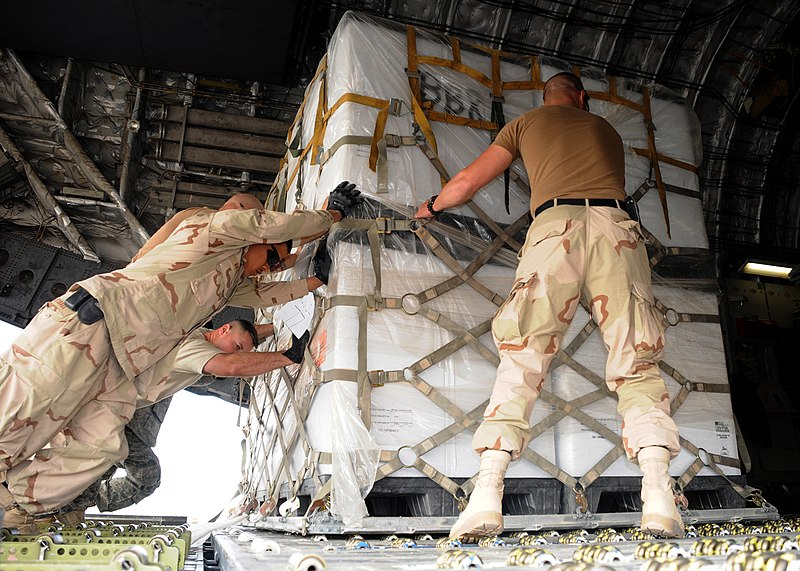
\includegraphics[scale=0.4]{Images/consolidated.jpg}
	\caption{Consolidated items on 463L pallets inside a {\it Boeing C-17}}
	\small\textsuperscript{Source: From Wikimedia Commons, the free media repository}
	\label{fig:larger2}
\end{figure}



\subsection{Aircraft and load balancing}


We consider real scenarios with a smaller or a larger aircraft with payloads of 26,000 kg or 75,000 kg respectively. Both layouts are represented in Figures \ref{fig:smaller} and \ref{fig:larger}, where the pallets are identified by $p_i$.

\begin{figure}[!h]
	\centering
	
	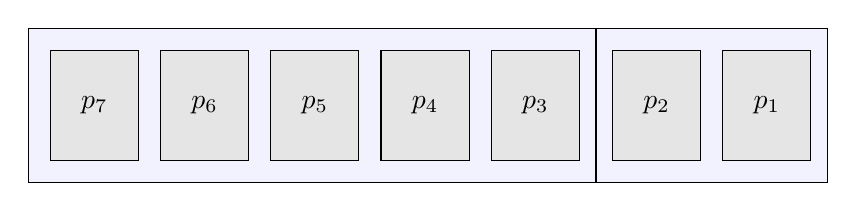
\begin{tikzpicture}[scale=1.4, samples=100]
		
		\filldraw[fill=blue!5!white, draw=black] (0, 0) rectangle (5.15, 1.4);
		\filldraw[fill=gray!20!white, draw=black] (0.2, 0.2) rectangle node{$p_7$} (1.0, 1.2); 
		\filldraw[fill=gray!20!white, draw=black] (1.2, 0.2) rectangle node{$p_6$} (2.0, 1.2); 
		\filldraw[fill=gray!20!white, draw=black] (2.2, 0.2) rectangle node{$p_5$} (3.0, 1.2); 
		\filldraw[fill=gray!20!white, draw=black] (3.2, 0.2) rectangle node{$p_4$} (4.0, 1.2); 
		\filldraw[fill=gray!20!white, draw=black] (4.2, 0.2) rectangle node{$p_3$} (5.0, 1.2); 
		\filldraw[fill=blue!5!white,  draw=black] (5.15,  0) rectangle             (7.25, 1.4);
		\filldraw[fill=gray!20!white, draw=black] (5.3, 0.2) rectangle node{$p_2$} (6.1, 1.2); 
		\filldraw[fill=gray!20!white, draw=black] (6.3, 0.2) rectangle node{$p_1$} (7.1, 1.2);	
		
	\end{tikzpicture}
	
	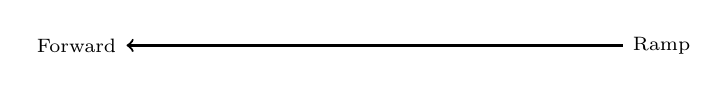
\begin{tikzpicture}[scale=1.4, samples=100]
		\draw[black, thick][<-]  (1, 2.17) node[anchor=east, font=\fontsize{7}{3.5}\selectfont]{Forward} -- (5.5, 2.17) node[anchor=west, font=\fontsize{7}{3.5}\selectfont]{Ramp} ;
	\end{tikzpicture}
	
	\caption{Smaller aircraft layout}
	%\small\textsuperscript{Source: the author}	
	\label{fig:smaller}
\end{figure}

\begin{figure}[!h]
	\centering
	
	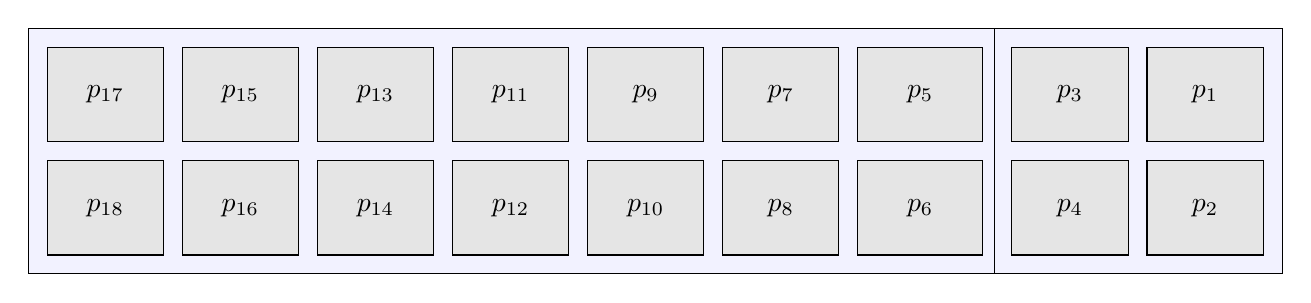
\begin{tikzpicture}[scale=1.2, samples=100]
		
		\filldraw[fill=blue!5!white, draw=black] (0, 0) rectangle (10.23, 2.6);
		
		\filldraw[fill=gray!20!white, draw=black] (0.20, 1.40) rectangle node{$p_{17}$} (1.43, 2.40);
		\filldraw[fill=gray!20!white, draw=black] (0.20, 0.20) rectangle node{$p_{18}$} (1.43, 1.20);
		
		\filldraw[fill=gray!20!white, draw=black] (1.63, 1.40) rectangle node{$p_{15}$} (2.86, 2.40);
		\filldraw[fill=gray!20!white, draw=black] (1.63, 0.20) rectangle node{$p_{16}$} (2.86, 1.20);
		
		\filldraw[fill=gray!20!white, draw=black] (3.06, 1.40) rectangle node{$p_{13}$} (4.29, 2.40);
		\filldraw[fill=gray!20!white, draw=black] (3.06, 0.20) rectangle node{$p_{14}$} (4.29, 1.20);
		
		\filldraw[fill=gray!20!white, draw=black] (4.49, 1.40) rectangle node{$p_{11}$} (5.72, 2.40);
		\filldraw[fill=gray!20!white, draw=black] (4.49, 0.20) rectangle node{$p_{12}$} (5.72, 1.20);
		
		\filldraw[fill=gray!20!white, draw=black] (5.92, 1.40) rectangle node{$p_{9}$} (7.15, 2.40);
		\filldraw[fill=gray!20!white, draw=black] (5.92, 0.20) rectangle node{$p_{10}$} (7.15, 1.20);
		
		\filldraw[fill=gray!20!white, draw=black] (7.35, 1.40) rectangle node{$p_{7}$} (8.58, 2.40);
		\filldraw[fill=gray!20!white, draw=black] (7.35, 0.20) rectangle node{$p_{8}$} (8.58, 1.20);
		
		\filldraw[fill=gray!20!white, draw=black] (8.78, 1.40) rectangle node{$p_{5}$} (10.1, 2.40);
		\filldraw[fill=gray!20!white, draw=black] (8.78, 0.20) rectangle node{$p_{6}$} (10.1, 1.20);
		
		\filldraw[fill=blue!5!white, draw=black] (10.23, 0) rectangle (13.27, 2.6);
		\filldraw[fill=gray!20!white, draw=black] (10.41, 1.40) rectangle node{$p_{3}$} (11.64, 2.40);
		\filldraw[fill=gray!20!white, draw=black] (10.41, 0.20) rectangle node{$p_{4}$} (11.64, 1.20);
		\filldraw[fill=gray!20!white, draw=black] (11.84, 1.40) rectangle node{$p_{1}$} (13.07, 2.40);
		\filldraw[fill=gray!20!white, draw=black] (11.84, 0.20) rectangle node{$p_{2}$} (13.07, 1.20);
		
	\end{tikzpicture}
	
	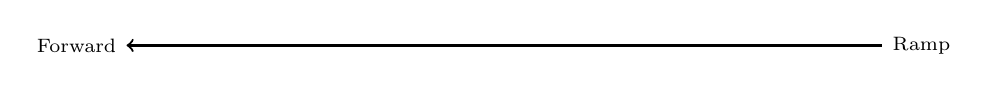
\begin{tikzpicture}[scale=1.2, samples=100]
		\draw[black, thick][<-]  (1, 2.77) node[anchor=east, font=\fontsize{7}{3.5}\selectfont]{Forward} -- (9, 2.77) node[anchor=west, font=\fontsize{7}{3.5}\selectfont]{Ramp} ;
	\end{tikzpicture}
	
	
	\caption{Larger aircraft layout} \label{fig:larger}
\end{figure}

In both cases, the torque applied to the aircraft must keep its CG in the operational range, which corresponds to a percentage of the {\it Mean Aerodynamic Chord} \footnote{Chord is the distance between the leading and trailing edges of the wing, measured parallel to the normal airflow over the wing \cite[p.18]{HoughtonCarpenter2003}. The average length of the chord is known as the {\it Mean Aerodynamic Chord} (MAC).}: $0.556m$ in the smaller aircraft and $1.17m$ in the larger one. See Figure \ref{fig:lateral}.

\begin{figure}[H]
	\centering
	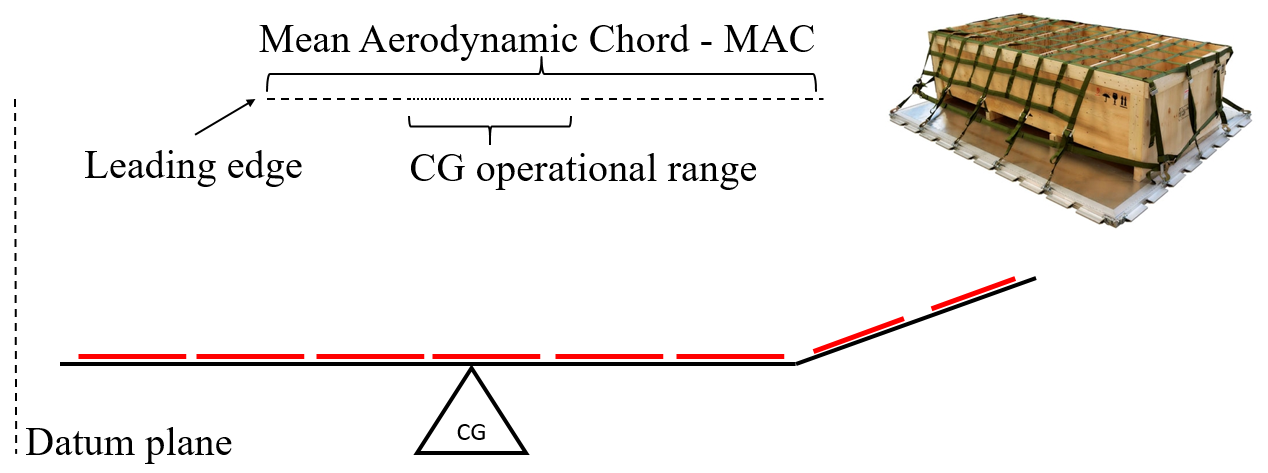
\includegraphics[scale=0.24]{Images/lateral.png}
	\caption{Aircraft longitudinal cut showing red lines as pallets}
	%\small\textsuperscript{Source: the author}
	\label{fig:lateral}
\end{figure}

Tables \ref{tab:smaller} and \ref{tab:larger} show the parameters in both cases. {\it CGx} and {\it CGy} refer to the relative distances of pallet centroids (in meters) in relation to the CG of aircraft along both axes. In both aircraft, as the ramps have an inclination of 25 degrees, we made the necessary corrections in {\it CGx}, {\it Weight} and {\it Volume limits} of the corresponding pallets. The monetary costs of both aircraft are also indicated: per unit of distance in flights between legs ($c_d$) and per deviation in the CG ($c_g$). It is important to consider that $c_g$ tends to zero as the aircraft attitude tends to level.


\begin{table}[H]
	\centering
	\caption{Smaller aircraft parameters}  \label{tab:smaller}
	\footnotesize
	\begin{tabular}{c | c c c c c c c}
		\toprule
		\bf {Limits}  & \multicolumn{3}{c}{$Payload$: $26,000kg$} & \multicolumn{4}{c}{$limit^{CG}_{long}$: $0.556m$} \\
		\midrule
		\bf {Pallets} & $p_7$ & $p_6$ & $p_5$ & $p_4$ & $p_3$ & $p_2$ & $p_1$ \\
		\midrule
		{\bf CGx ($m$)}     & -5.10 & -2.70 & -0.30   & 2.10 & 4.50 & 6.25 & 8.39  \\
		\midrule
		{\bf Weight limits ($kg$)}  & 4,500  &  4,500 &  4,500   & 4,500 & 4,500 & 4,000 & 3,500 \\ 
		{\bf Volume limits ($m^3$)} & 13.7  &  13.7 &  13.7   & 13.7 & 13.7 & 8.9 & 6.9 \\ 
		\midrule

		\bf {Costs}  & \multicolumn{4}{c}{$c_d$: US\$ $1.100/km$ } &	\multicolumn{3}{c}{$c_g = 0.05$} \\

		\bottomrule
	\end{tabular}
	\normalsize 
\end{table}


\begin{table}[H]
	\centering
	\caption{Larger aircraft parameters}  \label{tab:larger}
	\footnotesize
	\begin{tabular}{c | c c c c c c c c c}
		\toprule
		\bf {Limits}& \multicolumn{3}{c}{$Payload$: $75,000kg$} & \multicolumn{3}{c}{$limit^{CG}_{long}$: $1.170m$} &
		\multicolumn{3}{c}{$limit^{CG}_{lat}$: $0.19m$} \\
		\midrule
		\multirow{2}{*}{\bf {Pallets}}  & $p_{17}$ & $p_{15}$ & $p_{13}$ & $p_{11}$ & $p_{9}$ & $p_{7}$ & $p_{5}$ & $p_{3}$ & $p_{1}$ \\
		& $p_{18}$ & $p_{16}$ & $p_{14}$ & $p_{12}$ & $p_{10}$ & $p_{8}$ & $p_{6}$ & $p_{4}$ & $p_{2}$ \\
		\midrule 
		\multirow{2}{*}{\bf {CGx ($m$)}} & -17.57 & -13.17 & -8.77 & -4.40 & 0 & 4.40 & 8.77 & 11.47 & 14.89 \\
		& -17.57 & -13.17 & -8.77 & -4.40 & 0 & 4.40 & 8.77 & 11.47 & 14.89 \\			
		\midrule 
		\multirow{2}{*}{\bf {CGy ($m$)}}  & 1.32 & 1.32 & 1.32 & 1.32 & 1.32 & 1.32 & 1.32 & 1.32 & 1.32 \\
		& -1.32 & -1.32 & -1.32 & -1.32 & -1.32 & -1.32 & -1.32 & -1.32 & -1.32 \\	
		\midrule
		{\bf Weight limits ($kg$)}      &   4,500   &    4,500  &   4,500   &  4,500    & 4,500     & 4,500     & 4,500     & 4,000    & 3,000   \\
		{\bf Volume limits ($m^3$)}   &   14.8   &   14.8   &  14.8    &  14.8    & 14.8     & 14.8     & 14.8     & 10.0    & 7.0 \\	
		\midrule	

		\bf {Costs}  & \multicolumn{5}{c}{ $c_d$: US\$ $4.900/km$ } &	\multicolumn{4}{c}{$c_g = 0.05$} \\

		\bottomrule
	\end{tabular}
	\normalsize 
\end{table}

We accept the same assumptions as stated by \cite{MesquitaSanches2023}:
\begin{itemize}
	\item on each pallet, the items are distributed in such a way that their CG coincides with the centroid of the pallet;
	\item the CG of the payload must be at a maximum longitudinal distance of $limit^{CG}_{long}$ from the CG of the aircraft;
	\item in the larger aircraft, the CG of the payload must be at a maximum lateral distance of $limit^{CG}_{lat}$ from the CG of the aircraft;
	\item in the larger aircraft, pallets are distributed in two identical rows (with odd and even indices, respectively), and their centroids are at a distance $d^{CG}_{pallet}$ from the center-line of the aircraft.
\end{itemize}

\subsection{Problem Summary}

\newcolumntype{M}{>{\raggedright}p{0.03\textwidth}}
\newcolumntype{T}{>{\raggedright\arraybackslash}p{0.9\textwidth}}

\bgroup
\def\arraystretch{1.2}
\begin{table}[H]
	\centering
	\small
	\begin{tabular}{MT}
		&Informally, ACLP+RPDP can be summarized as follows:\\
		\midrule
		max &  (items score sum) / (tour cost) of picked up and delivered items on a tour  \\
		\midrule
s.t.    & Along a tour, the set of unvisited nodes is updated. \\
		& In each node, an item may be included in at most one pallet.\\		
		& In each node, consolidated items are composed of items with the same destination. \\
		& Weight, volume and score of a consolidated item are the corresponding sum of their components.\\
		& Consolidated items remain on board until their destinations.\\	
		& Consolidated items can only be included in the same pallet if their destinations are the same.\\
		& Only items destined for the remaining nodes can be loaded.  \\
		& The lateral and longitudinal torques must be within the operational range of the aircraft.\\
		& Weight and volume limitations of pallets must be respected.\\
		& The total weight must be less than the aircraft payload or the total pallet capacity, whichever is the lowest.\\	
		& The pallets destined for the next node of the tour should be put as near as possible to the cargo ramp door (our inclusion).\\		
		\midrule
	\end{tabular}
	\normalsize
\end{table}
\egroup 


\section{The mathematical modelling}
\label{sec4}

Given the assumptions, scenarios and parameters described in the previous section, we are ready to present the mathematical modelling of ACLP+RPDP, which is one of the contributions of our work.

Let $L = \{ l_0, l_1, \ldots, l_K \}$ be the set of $K+1$ nodes (or destinations), where $l_0$ is the origin and end of a flight plan. Let $d(l_i,l_j)$ be the distance from $l_i$ to $l_j$, where $0 \leq i,j \leq K$. By definition, $d(l_i,l_i)=0$. Let $L_k$ be the set of remaining nodes when the aircraft is in $l_k$, $0 \leq k \leq K$. Therefore, $L_0=L$ and $L_K = \{ l_0 \}$.

Let $C=\{c_{ij}\}$ be the cost matrix of flights, where $c_{ij} = c_d*d(l_i,l_j), 0 \leq i,j \leq K$.

Let $S_K = \{s: \{1, \dots, K\} \rightarrow \{1, \dots, K\} \}$ be the set of $K!$ permutations, which correspond to all possible tours (or itineraries) that have $l_0$ as origin and end, passing through the others $K$ nodes.

Let $M = \{p_1, p_2, \ldots, p_m \}$ the set of $m$ pallets. Each pallet $p_i$, $1 \leq i \leq m$, has weight capacity $p_i.w$, volume capacity $p_i.v$, pallet destinations $p_i.to[k]$, $0 \leq k \leq K$, and distance to the CG of aircraft $p_i.d$. $p_i.to[k]$ denotes that pallet $p_i$ may assume a different destination in each node $k$.

Let $N_k = \{t^k_1, t^k_2, \ldots, t^k_{n_k} \}$ be the set of $n_k$ items to be loaded in node $l_k$, $0 \leq k \leq K$. Each item $t^k_j$, $1 \leq j \leq n_k$, has score $t^k_j.s$, weight $t^k_j.w$, volume $t^k_j.v$, and destination $t^k_j.to \in L_k$. Let $N = \bigcup_{0 \leq k \leq K} N_k$ be the set of items of all nodes along a tour.

Let $Q_k = \{a^k_1, a^k_2, \ldots, a^k_{m_k} \}$ be the set of consolidated items loaded in $m_k \leq m$ pallets when the aircraft arrives at node $l_k$, with $0 \leq k \leq K$. $a^k_i$, $1 \leq i \leq m_k$, is the group of picked-up items that were allocated on pallet $p_i$ in some of the previous nodes. $a^k_i$ has total weight $a^k_i.w$, total volume $a^k_i.v$, and destination $a^k_i.to \in L_k \cup \{l_k\}$. If $a^k_i.to = l_k$, then $a^k_i$ is unloaded, and $p_i$ will be available for reloading; otherwise, $a^k_i$ remains on the aircraft, eventually in another pallet, and with items of $N_k$ having the same destination.

Let $X_{ij}^k$ and $Y_{iq}^k$ be binary variables, where $0 \leq k \leq K$, $1 \leq j \leq n_k$, $1 \leq i \leq m$ and $1 \leq q \leq m_k$. $X_{ij}^k = 1$ if $t_j^k$ is assigned to $p_i$ in node $l_k$, and 0 otherwise. $Y_{iq}^k = 1$ if $a_q^k$ is assigned to $p_i$ in node $l_k$, and 0 otherwise. By definition, $Y_{iq}^0=0$. Allocations of items or consolidated items to pallets in node $l_k$ can be seen as a bipartite graph $G_k(V_k, E_k)$, where $V_k = M \cup N_k \cup Q_k$, $E_k = E^N_k \cup E^Q_k$, $(p_i, t_j^k) \in E^N_k$ if $X_{ij}^k = 1$, and $(p_i, a_q^k) \in E^Q_k$ if $Y_{iq}^k = 1$.

The mathematical modeling of this problem is described in the equations below.


\begin{equation} \label{eq:maxf}
	\max_{\pi \in S_K} f_\pi(\tilde{s},\tilde{c})
\end{equation}

\begin{equation} \label{eq:scores}
	\tilde{s} = \sum_{k=0}^{K} \sum_{i=1}^{m} \sum_{j=1}^{n_k} X_{ij}^k \times t_j^k.s
\end{equation}

\begin{equation} \label{eq:costs}
	\tilde{c} = c_{0,\pi(1)}\times(1+c_g\times|\epsilon_0|) + \sum_{k=1}^{K-1} [ c_{\pi(k), \pi(k+1)}\times(1+c_g\times|\epsilon_k|) ] + c_{\pi(K),0}\times(1+c_g\times|\epsilon_K|)
\end{equation}

\begin{equation} \label{eq:maxW}
	maxW = \min(Payload, \sum_{i=1}^{m}p_i.w)
\end{equation}

\begin{equation} \label{eq:tau}
\tau_k = \sum_{i=1}^{m}[ p_i.d \times (\sum_{j=1}^{n_k} X_{ij}^k \times t_j^k.w +  \sum_{q=1}^{m} Y_{iq}^k \times a_q^k.w)];\ k \in \{0, 1, \ldots, K\}
\end{equation}

\begin{equation} \label{eq:eps}
\epsilon_k = \frac{\tau_k}{maxW \times limit^{CG}_{long}};\ k \in \{0, 1, \ldots, K\}
\end{equation}

\begin{equation} \label{eq:pdp11}
	L_0 = L; L_{k} = L_{k-1} - \{l_{\pi(k)}\}; \ k \in \{1, 2, \ldots, K\}
\end{equation}

\begin{equation} \label{eq:pdp13}
	Y^0_{iq} = 0; a^0_i.w = 0; a^0_i.v = 0; a^0_i.to = -1;\ i,q \in \{1, 2, \ldots, m\}
\end{equation}

\begin{equation} \label{eq:pdp12}
	X_{ij}^k = 0 \ \mbox{if} \ t_j^k.to \notin L_k; \ i \in \{1, 2, \ldots, m\}; \ j \in \{1, 2, \ldots, n_k\}; \ k \in \{1,2, \ldots, K\}
\end{equation}

\begin{equation} \label{eq:pdp9}
	Y_{iq}^k = 0 \ \mbox{if} \ a_i^k.to \notin L_k; \ i \in \{1, 2, \ldots, m\}; \ q \in \{1, 2, \ldots, m_k\}; \ k \in \{ 1, 2, \ldots, K\}
\end{equation}

\begin{equation} \label{eq:cons2}
	a_i^{\pi(k+1)}.w = \sum_{j=1}^{n_k} X_{ij}^{\pi(k)} \times t_j^{\pi(k)}.w + \sum_{q=1}^{m_k} Y_{iq}^{\pi(k)} \times a_q^{\pi(k)}.w;  \ i \in \{1, 2, \ldots, m_k\}; k \in \{0, 1, \ldots, K-1\}
\end{equation}

\begin{equation} \label{eq:cons3}
	a_i^{\pi(k+1)}.v = \sum_{j=1}^{n_k} X_{ij}^{\pi(k)} \times t_j^{\pi(k)}.v + \sum_{q=1}^{m_k} Y_{iq}^{\pi(k)} \times a_q^{\pi(k)}.v;  \ i \in \{1, 2, \ldots, m_k\}; k \in \{0, 1, \ldots, K-1\}
\end{equation}

\begin{equation} \label{eq:cons5}
	a_i^{\pi(k+1)}.to = t^{\pi(k)}_j.to  \ \mbox{if} \ X^{\pi(k)}_{ij} = 1  \ \mbox{and} \ t^{\pi(k)}_j.to \in L_{k+1};  \ i \in \{1, 2, \ldots, m_k\}; \ j \in \{1, 2, \ldots, n_k\}; \ k \in \{0,1, \ldots, K-1\}
\end{equation}

\begin{equation} \label{eq:LatIt}
	LatIt_k = \sum_{i=1}^{m} \sum_{j=1}^{n_k} ( X_{ij}^k \times t_j^k.w \times (i\%2) - X_{ij}^k \times t_j^k.w \times (i+1)\%2 ); \ k \in \{0, 1, \ldots, K\}
\end{equation}

\begin{equation} \label{eq:LatCons}
	LatCons_k =  \sum_{i=1}^{m} \sum_{q=1}^{m_k}  ( Y_{iq}^k \times a_q^k.w \times (i\%2) - Y_{iq}^k \times a_q^k.w \times (i+1)\%2); \ k \in \{0, 1, \ldots, K\}
\end{equation}

\begin{equation} \label{eq:torqlat}
	s.t.: d^{CG}_{pallet} \times | LatIt_k + LatCons_k | \leq  \sum_{i=1}^{m}p_i.w \times limit^{CG}_{lat}; \ k \in \{0, 1, \ldots, K\}
\end{equation}

\begin{equation} \label{eq:torqlong}
	s.t.: |\tau_k| \leq maxW \times limit^{CG}_{long};\ k \in \{0, 1, \ldots, K\}
\end{equation}

\begin{equation} \label{eq:payload}
	s.t.: \sum_{i=1}^{m} (\sum_{j=1}^{n_k} X_{ij}^k \times t_j^k.w + \sum_{q=1}^{m_k} Y_{iq}^k \times a_q^k.w ) \leq maxW; \ k \in \{0, 1, \ldots, K\}
\end{equation}

\begin{equation} \label{eq:app2}
	s.t.: \sum_{j=1}^{n_k} X_{ij}^k \times t_j^k.w + \sum_{q=1}^{m_k} Y_{iq}^k \times a_q^k.w  \leq p_i.w; \ i \in \{1, 2, \ldots, m_k\}; \ k \in \{0, 1, \ldots, K\}
\end{equation}

\begin{equation} \label{eq:app3}
	s.t.: \sum_{j=1}^{n_k} X_{ij}^k \times t_j^k.v + \sum_{q=1}^{m_k} Y_{iq}^k \times a_q^k.v  \leq\ p_i.v; \ i \in \{1, 2, \ldots, m_k\}; \ k \in \{0, 1, \ldots, K\}
\end{equation}

\begin{equation} \label{eq:app4}
	s.t.: \sum_{i=1}^{m} X_{ij}^k \leq 1; \ j \in \{1, 2, \ldots, n_k\}; \ k \in \{0, 1, \ldots, K\}
\end{equation}

\begin{equation} \label{eq:app5}
	s.t.:  Y_{iq}^k = 1 \ \mbox{if} \ a^k_q.to \in L_k; \ q \in \{1, 2, \ldots, m_k\}; \ k \in \{0, 1, \ldots, K\}
\end{equation}

\begin{equation} \label{eq:pdp8}
	s.t.: p_i.to[k] = t^k_j.to\ \mbox{if} \ X_{ij}^k = 1; \ i \in \{1, 2, \ldots, m\}; \ j \in \{1, 2, \ldots, n_k\}; \ k \in \{1, 2, \ldots, K\}
\end{equation}

\begin{equation} \label{eq:pdp2}
	s.t.:  p_i.to[k] = a^k_q.to\ \mbox{if} \ Y_{iq}^k = 1; \ i \in \{1, 2, \ldots, m\};\ q \in \{1, 2, \ldots, m_k\}; \ k \in \{1, 2, \ldots, K\}
\end{equation}


The objective of this problem is to find a permutation $\pi \in S_K$\/ that maximizes the function $f_\pi(\tilde{s},\tilde{c})$ \ref{eq:maxf}. In this way, the flight plan will be $l_0, l_{\pi(1)}, \ldots, l_{\pi(K)}, l_0$. $\tilde{s}$\/ is the total score of transported items \ref{eq:scores} and  $\tilde{c}$\/ is the total cost of fuel consumed \ref{eq:costs}. As can be seen, $\tilde{c}$\/ corresponds to the fuel consumption due to the flights carried out and the CG deviation of the transported cargo. Throughout this work, for simplicity, we use $f=\tilde{s}/\tilde{c}$.

The maximum load will be the minimum between the payload and the capacity supported by the pallets \ref{eq:maxW}. Considering the maximum longitudinal distance allowed for the CG, all torques \ref{eq:tau} and deviations \ref{eq:eps} are calculated.

For each step of the flight plan, the set of unvisited nodes is updated \ref{eq:pdp11}. Although there are no items consolidated at the beginning of the flight plan, we defined these variables for ease of notation \ref{eq:pdp13}. Items destined outside the rest of the flight plan will not be loaded (\ref{eq:pdp12} and \ref{eq:pdp9}).

Consolidated items appear when there are items on the pallets that will not be unloaded on the next node. Its weights \ref{eq:cons2} and volumes \ref{eq:cons3} correspond to all the items that were on the pallet, since all these items have the same destination. On subsequent nodes, consolidated items can be allocated with other items of same destination \ref{eq:cons5}.

Equations \ref{eq:LatIt} and \ref{eq:LatCons} respectively, are applied only to the larger aircraft, and calculate the lateral torques of items and consolidated items loaded in both rows of pallets, whose constraint is described in \ref{eq:torqlat}. Similarly, \ref{eq:torqlong} is the longitudinal torque constraint, which is applied to both aircraft sizes.

The weight limitation of the aircraft must be respected \ref{eq:payload}. The sum of weights \ref{eq:app2} and volumes \ref{eq:app3} in each pallet must not exceed its capacity. Each item is associated with a pallet at most \ref{eq:app4}.

Consolidated items remain on board \ref{eq:app5} until their destinations. At each node, an item (\ref{eq:pdp8}) and a consolidated item (\ref{eq:pdp2}) must only be allocated to a pallet if the destinations are the same.


\section{Resolution strategy}
\label{sec5}

Once the assumptions of this work and the mathematical modelling of the problem are presented, it is easy to see that ACLP+RPDP is NP-hard. In a similar way to \cite[p. 6]{LurkinSchyns2015}, consider the simple case where $K=1$\/ (one leg), $m=2$ (two pallets around the aircraft CG), $2n$\/ sufficiently light items with same scores in $l_0$, and no items in $l_1$. Under these conditions, through polynomial reductions for the {\it Set-Partition Problem}, it is possible to demonstrate that the decision problem associated with ACLP+RPDP is NP-complete.

Real cases are more complex as they have hundreds of different items in each node and involve three intractable sub-problems: APP, WBP and SPDP. Through the mathematical modelling presented in the previous section, we verify that {\it Mixed-Integer Programming}\/ (MIP) is not able to solve these cases in feasible time. Thus, it is necessary to adopt some strategy to find a viable solution, not necessarily optimal, that seeks to maximize the objective function $f$.

\cite{MesquitaSanches2023} strategy is based on the fact that, in real cases, $K$\/ is usually small. Specifically, they will consider $K \leq 6$\/ throughout their and our work, which is a higher value than usual in {\it Brazilian Air Force} missions. As a result, if we have fast node-by-node solutions that allow us to construct a complete tour, we will be able to test all possible $K!$\/ tours and thus select the one that provides the best value for the $f$\/ function.

The tactic will be, at each shipping node, to predefine the destinations of the pallets at that node. In this way, we will reserve a number of pallets proportional to the volume demanded by each destination at the shipping node. We could have used another criterion, but it was observed in the experiments that volume is more constrictive in airlift. Once the destinations of the pallets are defined, we will use serial and Multi-processing heuristics to find the best possible node-by-node solutions. This strategy is summarized in Algorithm \ref{alg:main}, retrieved from \cite{MesquitaSanches2023}.


\begin{algorithm}[H]
	\caption{Solves ACLP+RPDP for a scenario with certain volume surplus (1.2, 1.5, or 2.0)}  \label{alg:main}
	\begin{algorithmic}[1]
		
		\Procedure{$ACLP+RPDP$}{$scenario,\ surplus,\ numProcs,\ timeLim$}
		
		\State Let $L, M, C$ be according to $scenario$ \label{main:LMC}
		\State $N \gets ItemsGeneration(scenario,\ surplus)$ \label{main:items}
		\For {each $method$}
				
			\For {each $\pi \in S_K$} \label{main:loop1}
				\State $f_{\pi} \gets SolveTour(\pi, L, M, C, N, method, numProcs,\ timeLim )$ \label{main:method}
			\EndFor \label{main:loop2}
			\State $answer[scenario,surplus,method] \gets \max f$ \label{main:f}
		\EndFor
		
		\Return $answer$
		
		\EndProcedure
	\end{algorithmic}
\end{algorithm}


In this algorithm, there are six values for the $scenario$\/ parameter, according to Table \ref{tab:scenarios}, which defines $K$, the sets of nodes, the aircraft, the pallets and the costs from Tables \ref{tab:smaller} or \ref{tab:larger} that will be used (line \ref{main:LMC}).


The other parameter $volume$\/ is a value greater than 1, which corresponds, at each node $l_k$, to the ratio between the sum of the volumes of the items ($\sum_{j=1}^{n_k} t^k_j.v$) and the load capacity of the pallets ($\sum_{i=1}^{m} p_i.v$). This parameter is passed to $ItemsGeneration$ (line \ref{main:items}), responsible for creating the items to be shipped, which will be presented in the next section.

$method$\/ corresponds to one of the heuristics that we will present in subsection \ref{methods}. The loop of lines \ref{main:loop1}-\ref{main:loop2} goes through all permutations $\pi$, where the node-by-node resolutions are performed by $SolveTour$, whose result is stored in $f_{\pi}$. The best result among all $K!$\/ tours will be the answer for $scenario$, $volume$\/ and $method$\/ (line \ref{main:f}). 

\vspace{2.0mm}
\begin{table}[H]
	\centering
	\caption{Testing scenarios retrieved from \cite{MesquitaSanches2023}.}  \label{tab:scenarios}
	\begin{tabular}{c c c c }
		\toprule
		{\bf Scenario} & {$K$} & {$L$} & {\bf Aircraft} \\		
		\midrule
		1 & 2    & \{$l_0$, $l_1$, $l_2$\}                                 & smaller \\
		2 & 2    & \{$l_0$, $l_1$, $l_2$\}                                 & larger  \\
		3 & 3    & \{$l_0$, $l_1$, $l_2$, $l_3$\}                          & larger  \\
		4 & 4    & \{$l_0$, $l_1$, $l_2$, $l_3$, $l_4$\}                   & larger  \\
		5 & 5    & \{$l_0$, $l_1$, $l_2$, $l_3$, $l_4$, $l_5$\}            & larger  \\
		6 & 6    & \{$l_0$, $l_1$, $l_2$, $l_3$, $l_4$, $l_5$, $l_6$\}     & larger  \\
		\bottomrule
	\end{tabular}
\end{table}

Next, we will present two subsections: in the first we explain how $SolveTour$ is executed, while in the second we will present the heuristics developed for node-by-node resolutions.


\subsection{SolveTour algorithm}
\label{tour}

In addition to the set of nodes, pallets, costs and items, $SolveTour$, described in Algorithm \ref{alg:tour}, receives the parameter $method$, which corresponds to a heuristic for solving the node-by-node problems, and the parameter $\pi$, which is a permutation that defines the order of visits in this tour.

As we mentioned in the previous section, all tours start and end at $l_0$\/ (lines \ref{tour:pi1}-\ref{tour:pi2}).
After initializing the score and cost values (lines \ref{tour:score}-\ref{tour:cost}), there is a loop for the $K+1$\/ flights (lines \ref{tour:loop1}-\ref{tour:loop2}). Initially we set pallets destination as $-1$\/ (line \ref{tour:-1}). When the aircraft is at node $l_0$, the initial graph $G_1$\/ is empty because it has no consolidated items \ref{tour:g11}. Otherwise, the set $L_k$\/ of remaining nodes is updated (line \ref{tour:lk1}), and $UpdateConsolidated$\/ (line \ref{tour:dest}) returns the set of consolidated items that have not yet reached their destination and remain on board, rearranging them on the pallets to minimize CG deviation. This allocation is stored in graph $G_1$\/ (line \ref{tour:g12}).

In the context of this work, we know that $m>K$, once the aircraft has $7$\/ or $18$\/ pallets and $K\leq 6$, allowing there to be at least one pallet for each node to be visited. $SetPalletsDestination$\/ (line \ref{tour:dest2}) presets the destination of each pallet based on the volume demands of the current node, without changing the pallets destination with consolidated items.

Finally, $SolveNode$\/ includes the edges corresponding to the items shipped at the current node, returning the graph $G_2$\/ (line \ref{tour:node}). The score and the CG deviation of this graph are calculated (line \ref{tour:analyse}) and accumulated (lines \ref{tour:score2}-\ref{tour:cost2}), allowing the final result of this tour (line \ref{tour:f}).

\begin{algorithm}[H]
	\caption{ Solves the sequence of nodes in the tour indexed by $\pi$ }  \label{alg:tour}
	
	\begin{algorithmic}[1]
		
		\Procedure{$SolveTour$}{$\pi, L, M, C, N, method, numProcs,\ timeLim$}
		
		\State $\pi(0) \gets 0$ \label{tour:pi1}
		\State $\pi(K+1) \gets 0$ \label{tour:pi2}
		\State $score \gets 0$ \label{tour:score}
		\State $cost \gets 0$ \label{tour:cost}
		\For {$k\gets0$ to $K$} \label{tour:loop1}		
			\For{$i \gets 1$ to $m$}
				\State $p_i.to[k] \gets -1$ \label{tour:-1}
			\EndFor	
			\If {$k = 0$}
				\State $L_0 \gets L$
				\State Let $G_1(M \cup N_0, \varnothing)$ \label{tour:g11}
			\Else
				\State $L_k \gets L_k - \pi(k)$  \label{tour:lk1}			
				\State $Q_{\pi(k)}, E^Q_{\pi(k)}, M \gets UpdateConsolidated(\pi(k))$ \label{tour:dest}			
				\State Let $G_1(M \cup N_{\pi(k)} \cup Q_{\pi(k)}, E^Q_{\pi(k)})$ \label{tour:g12}
			\EndIf  \label{tour:lk2}	
			\State $M \gets SetPalletsDestination( \pi(k) )$ \label{tour:dest2}		
			\State $G_2 \gets SolveNode(method, \pi(k), G_1, numProcs,\ timeLim)$ \label{tour:node}
			\State $s, \epsilon \gets ScoreAndDeviation(\pi(k), G_2)$ \label{tour:analyse}
			\State $score \gets score + s$ \label{tour:score2}
			\State $cost \gets cost + c_{\pi(k),\pi(k+1)} * (1 + c_g * |\epsilon|)$ \label{tour:cost2} 
		\EndFor  \label{tour:loop2}
		\Return $score / cost$ \label{tour:f}
		
		\EndProcedure
		
	\end{algorithmic}
\end{algorithm}

$UpdateConsolidated$ finds the best allocation for the consolidated items that remain on board. Initially, the set $Q$ is created, with the consolidated items that did not reach their destination.

Then $MinCGDeviation$ is run through a MIP solver to relocate the consolidated items on the pallets minimizing torque and ensuring that they all remain on board, one on each pallet. As there are few variables, the MIP solver returns an allocation $E^Q_k$ very quickly.

$SetPalletsDestination$ sets pallets destination not yet defined. The total volume of items and the number of pallets with consolidated items destined for each node. The destinations of each pallet are defined proportionally to the volume of items, regarding the pallets with consolidated items.

$ScoreAndDeviation$ evaluates the allocation graph generated by $SolveNode$, returning the corresponding score and CG deviation. It consists of a loop that goes through all the pallets, accumulating the scores and the torques of the shipped items, allowing the final calculation of the CG deviation.

$UpdateConsolidated$, $MinCGDeviation$, $SetPalletsDestination$, and $ScoreAndDeviation$ are thoroughly described by \cite{MesquitaSanches2023}.


\subsection{Node-by-node solutions}
\label{methods}


In this subsection we present implementations of $SolveNode(method,k, G)$, where $method$\/ corresponds to a heuristic, $k$\/ is the index of the current node and $G$\/ is the allocation graph of the consolidated items that remain on board at node $l_k$.

An important issue on meta-heuristics is that they are known for the hard work in tuning parameters. For this, when we use the word {\it empirically}\/ throughout the text, we want to say that we accomplished many tests with the hardest instances to fit these values. This does not guarantee best results for all instances, but, on average, overall results are acceptable. Another important observation is that our {\it ACO} implementations were designed based on traditional ideas from the literature \cite{Fidanova2006} and on the experiences learned during tests, plus the special features to process-based parallelism.

To guarantee that performance comparisons are made correctly, our implementations use the same elements described below.

\newcolumntype{C}{>{\raggedright}p{0.19\textwidth}}
\newcolumntype{D}{>{\raggedright\arraybackslash}p{0.81\textwidth}}

\bgroup
\def\arraystretch{1.2}
\begin{table}[H]
	\centering
	\small
	\begin{tabular}{CD}
		
		{\it Data structure:}     & Items, pallets and edges are arrays of \emph{Python} class objects, which are initialized with the same data loaded from text files. \\
		
		{\it Stopping criterion:} & All methods have the same time limit of $0.7$ seconds per node.\\
		
		{\it Common procedures:}  & All methods have the same procedures for: solution printing, pallets destinations and initial parameters setting, solution integrity checking, and the same procedures for selecting and inserting edges.\\

	\end{tabular}
	\normalsize
\end{table}
\egroup

The selection of edges for $E^N_k$\/ uses the {\it edge attractiveness}\/ $\theta^k_{ij}$, Equation \ref{eq:edge}, which can be understood as the tendency to allocate the item $t^k_j$\/ to the pallet $p_i$. It is directly proportional to the score, and inversely proportional to the volume and the torque of each item. The 3000 value was empirically set to keep the attractiveness in the range [0, 1], to be in the same order of magnitude of the Ant Colony Optimization pheromone range.

\begin{equation} \label{eq:edge}
	\theta^k_{ij}= \frac{t^k_j.s}{t^k_j.v \times 3000}\times(1-\frac{t^k_j.w\times|p_i.d|}{\max_s\{t^k_s.w\}\times\max_q\{|p_q.d|\}});\ i \in \{1,2,\ldots,m\},\ j \in \{1,2,\ldots,n_k\}
\end{equation} 


We use four types of random selections:
\begin{itemize}
	\item $RandomReal(r_1,r_2)$: randomly selects a real number in $[r_1,r_2]$;
	\item $RandomInt(i_1,i_2)$: randomly selects a integer number in $[i_1,i_2]$;
	\item $Roulette(set)$ biased through $\phi$: selects an element from $set$, where the probability of each element is proportional to the value of a given function $\phi$\/ defined on $set$.
\end{itemize}


To compare allocation graphs generated by the heuristics, we choose the one that offer a higher associated score, since the CG deviation is limited by the constraints.

In the pseudo-codes presented below, given an allocation graph $G$\/ for the node $l_k$, $f_s(G)$\/ is equivalent to the score $s$\/ returned by $ScoreAndDeviation(k,G) $, described in \cite{MesquitaSanches2023}.

Below, we present 2 implementations for $SolveNode$: {\it Multi-process Ant Colony Optimization}\/ ({\it mpACO})  and a new parallel heuristic that we propose called {\it Multi-process Shims (mpShims)}.

According to \cite[p.226]{manfrin2006}, there are five topologies for multi-process interchange of information: {\it fully-connected}, where the master process broadcasts to all remaining child processes; {\it replace-worst}, where the best-so-far solution process broadcasts only to the current worst solution process; {\it hypercube}, where processes are connected as a hypercube, and a vertex process broadcasts only to the connected vertices; {\it ring}, in which one process only sends a message to the next process connected to it; and {\it parallel independent runs (PIR)}, in which there are no communication costs and the best solution is chosen among all processes. They concluded that the PIR topology presented, in average, the smallest distance from the optimal solutions.

It is important to say that the parallel ACO ({\it pACO}) is a different implementation where employs threads instead of processes to solve each ant solution in parallel (for a detailed information on parallel ACO see \cite{Pedemonte2011}). We chose {\it mpACO} for our approach because we employed the {\it Fully-Connected} topology which requires to share the pheromone array between the multi-process ants and the facility to handle the possibility of race condition.


\subsubsection{Multi-process Ant Colony Optimization (mpACO)}

In ACO \cite{Dorigo1992}, a population of $A$\/ ants performs independent search (sequential or in parallel), where each ant $a$\/ finds its own allocation graph $G^a$. Each edge $e^k_{ij}=(p_i,t^k_j)$\/ has a general attractiveness $ga^k_{ij} = (\tau^k_{ij})^\alpha + (\theta^k_{ij})^\beta$, where $\tau^k_{ij}$\/ is the pheromone of this edge, and $\alpha$\/ and $\beta$\/ are constants. If $e^k_{ij}$\/ is included in $G^a$, ant $a$\/ increases the pheromone $\tau^k_{ij}$.

Algorithm \ref{alg:aco} presents this heuristic in its parallel multi-process version as we have implemented.

$SolveNode(mpACO, k, G, numProcs)$ is the main process, while $AntSolve(G^+,\ AntsQueue,\ ga^k_{ij})$ is executed the child concurrent processes.

\begin{algorithm}[H] 
	
	
	\caption{ Solves a node with the {\it mpACO} method } \label{alg:aco}
	\begin{algorithmic}[1]
		
		\Procedure{$SolveNode$}{$mpACO, k, G, numProcs,\ timeLim$}
		
		\State Let $G(V_k, E^Q_k)$ \Comment{This is a partial solution with only consolidated on board}
		\State $G^*(V_k, E^{N*}_k \cup E^Q_k), \_ \gets Greedy(k, G, 0.9)$  \label{aco:greedy} \Comment{This partial solution is completed by a greedy algorithm}
		\State $G^+(V_k, E^{N+}_k \cup E^Q_k) \gets G^*(V_k,E^{N*}_k \cup E^Q_k)$
		\State $A \gets numProcs$ \label{aco:numProcs}
		\State $ga^k_{ij}   \gets 0$, $1 \leq i \leq m$, $1 \leq j \leq n_k$  \label{aco:init1}
		\State $\tau^k_{ij} \gets 1$, $1 \leq i \leq m$, $1 \leq j \leq n_k$   \label{aco:init2}
		\State $\alpha    \gets 1.0$ \label{aco:alpha}
		\State $\beta     \gets 4.0$ \label{aco:beta}
		\State $\rho      \gets 0.2$ \label{aco:rho}
		\State $stagnant \gets 0$
		\While{ $stagnant < 3$ } \label{aco:while}
					
			\State $AntsQueue \gets \{\ \}$ \label{aco:AntsQueue}

			\For{$1$ {\bf to} $A$} \label{aco:AntsSolve}	
				\State $AntSolve(G^+,\ AntsQueue,\ ga^k_{ij})$
			\EndFor
			
			\State $counter \gets A$
						
			\While{$counter > 0$} \label{aco:while2}
			
				\State $G^{a} \gets \varnothing$
			
				\While{$runtime < timeLim$} \Comment{Wait until there is a solution in the queue}
			
					\State $G^{a} \gets AntsQueue.Pop()$
					
					\If{$G^{a} \ne \varnothing$}				
						\Break
					\EndIf
				
				\EndWhile
					
				\If{$f_s(G^{a}) > f_s(G^{+})$}
					\State $G^+(V_k, E^{N+}_k \cup E^Q_k) \gets G^a(V_k, E^{Na}_k \cup E^Q_k)$ 
				\EndIf
				
				\State $counter \gets counter - 1$
												
			\EndWhile			
									
			\If{$f_s(G^+) > f_s(G^*)$} \label{aco:best1}
				\State $stagnant \gets 0$
				\State $G^*(V_k, E^{N*}_k \cup E^Q_k) \gets G^+(V_k, E^{N+}_k \cup E^Q_k)$		
			\Else
				\State $stagnant \gets stagnant + 1$ 
			\EndIf
			\For{all $\tau^k_{ij}$} 
				\State $\tau^k_{ij} \gets (1-\rho)\tau^k_{ij}$ \label{aco:rho2}
				\State $\tau^k_{ij} \gets \tau^k_{ij} + \Delta\tau$ \label{aco:phero2}
				\State $ga^k_{ij} \gets (\tau^k_{ij})^\alpha + (\theta^k_{ij})^\beta$ \label{aco:ga2}				
			\EndFor	
		\EndWhile	
		\Return $G^*(V_k,\ E^{N*}_k \cup E^Q_k)$
		
		\EndProcedure		
	\end{algorithmic}
\end{algorithm}
	
A greedy solution is obtained in line \ref{aco:greedy}, being initially stored in $G^*$\/ and $G^+$. The argument 0.9 generates an initial and poor solution for ACO to improve. The second return value denoted by underscore is not used by ACO.

The number $A$\/ of ants was set to the number of parallel processes (line \ref{aco:numProcs}).

The $m \times n_k$\/ matrices $\tau^k_{ij}$ and $ga^k_{ij}$\/ (lines \ref{aco:init1}-\ref{aco:init2}) are used and updated by all ants. For further explanation, see \cite{DorigoManiezzoColorni1996}. 

The number of iterations depends on the time limit or stagnation in improving results (line \ref{aco:while}).
At the beginning os each iteration (\ref{aco:AntsQueue}) a queue of ants ($AntsQueue$) is created to hold ants parallel solutions generated in the child processes.

The local solution $G^+$ is sent to A child processes (\ref{aco:AntsSolve}) almost simultaneously.
While there are any ant working on an solution or the run-time is still less then maximum (\ref{aco:while2}), it hangs in the $AntsQueue$ until there is a solution available.

If there is a global improvement (\ref{aco:best1}) the best so far solution ($G^*(V_k, E^{N*}_k \cup E^Q_k)$) is updated.
At the end of each iteration pheromone levels (\ref{aco:rho2}) are evaporated, than updated with the new calculated $\Delta\tau$ (line \ref{aco:phero2}), and according to Equation \ref{eq:delta_tau}, and the general attractiveness ( \ref{aco:ga2}) is also updated.

\begin{equation} \label{eq:delta_tau}
	\Delta\tau = \frac{f_s(G^{+}) - f_s(G^{*})}{A \times f_s(G^{*})}
\end{equation}

Many ACO applications update pheromone levels and the general attractiveness only when there is a solution improvement. Differently, this work updates in both cases, exploring also the negative learning approach proposed by \cite{math9040361}. We did not compare these performances because it is out of the scope of this work.


We also developed Algorithm \ref{alg:greedy}, which generates a greedy allocation of the items available in node $l_k$, according to the non-ascending order of $\theta^k_{ij}$, and considering the consolidated items already shipped ($E^Q_k$). Edges are included in this allocation as long as they respect feasibility constraints. Furthermore, the volume of each pallet $p_i$\/ cannot exceed $p_i.v \times limit$, where $ 0 < limit \leq 1$\/ is a given parameter.

\begin{algorithm}[H]
	\caption{Mount a greedy solution until the volume limit for each pallet}  \label{alg:greedy}
	
	\begin{algorithmic}[1]
		
		\Procedure{$Greedy$}{$k, G, limit$}
		
		\State Let $G(V_k, E^Q_k)$
		
		\State $\eta_1 \gets \{0\} \times m$ \label{greedy:eta}
		\State $volume \gets \{0\} \times m$
		
		\State $E^N_k \gets \varnothing$ 			
		
		\For{$q \gets 1$ to $m$}
			\If{$(p_i, a_q^k) \in E^Q_k$} 
				\State $volume[q] \gets volume[q] + a_q^k.v$ 
			\EndIf		
		\EndFor
			
		\For {each $e_{ij}^k$ in non-ascending order of $\theta^k_{ij}$}
			\If{($E^N_k \cup \{e_{ij}^k\}$ is feasible) {\bf and} ($volume[i] \leq p_i.v \times limit$)} 
				\State $E^N_k \gets E^N_k \cup \{e_{ij}^k\}$ 
				\State $volume[i] \gets volume[i] + t_j^k.v$
				\State $\eta_1[i] \gets \eta_1[i] + 1$ 	
			\EndIf
		\EndFor
		
		\Return $G(V_k, E^N_k \cup E^Q_k),\ \eta_1$ \Comment{return the solution and the last item indexes array }
		
		\EndProcedure
		
	\end{algorithmic}
\end{algorithm}

In Algorithm \ref{alg:greedy}, line \ref{greedy:eta} defines an array with the same size as pallets array to save the set of last edges inserted in the greedy solution. The set $\eta_1$ is returned together with the greedy solution.


\begin{algorithm}[H] 
	\caption{Each ant solves a node in parallel} \label{alg:AntSolve}
	\begin{algorithmic}[1]
		
		\Procedure{$AntSolve$}{$G^+,\ AntsQueue,\ ga^k_{ij})$}
		
		\State $G^a(V_k, E^{Na}_k \cup E^Q_k) \gets G^+(V_k, E^{N+}_k \cup E^Q_k)$
		\State $E \gets \{ (p_i,t^k_j) \mid (p_i,t^k_j) \not\in E^{Na}_k \}$ \label{AntSolve:neighborhood}
		\While{$|E| > 0$} \label{AntSolve:not_empty}
		
			\State $e \gets Roulette(E)$ biased through $ga^k_{ij}$  \label{AntSolve:roulette}
			\State $E \gets E - \{e\}$		
			\If{$E^{Na}_k \cup \{e\}$ is feasible}
				\State $ E^{Na}_k \gets E^{Na}_k \cup \{e\} $ \label{AntSolve:ant}
			\EndIf
			
		\EndWhile
		
%\For{$\tau^k_{ij}, \theta^k_{ij} \in E^{Na}_k$}
%\State $\tau^k_{ij} \gets (1-\rho)\tau^k_{ij}$ \label{AntSolve:rho}
%\State $\tau^k_{ij} \gets \tau^k_{ij} + \Delta\tau$ \label{AntSolve:phero}  \Comment{$\Delta\tau \gets$ Equation \ref{eq:delta_tau}}
%\State $ga^k_{ij} \gets (\tau^k_{ij})^\alpha + (\theta^k_{ij})^\beta$ \label{AntSolve:ga}		
%\EndFor
		
		\State $AntsQueue \gets AntsQueue \cup G^a(V_k,\ E^{Na}_k \cup E^Q_k)$ \label{AntSolve:put_in_queue}
		
		\EndProcedure
	\end{algorithmic}
\end{algorithm}

Algorithm \ref{alg:AntSolve}, which will be executed by a child parallel process, receives an initial and poor solution $G^+(V_k, E^{N+}_k \cup E^Q_k)$ generated greedily to be completed and improved by {\it mpACO}.

Line \ref{AntSolve:neighborhood} expresses the creation of the neighborhood, the set of candidate edges.

While the neighborhood is not empty (line \ref{AntSolve:not_empty}), choose an edge (line \ref{AntSolve:roulette}), delete it from the neighborhood and include it in the solution, if feasible (line \ref{AntSolve:ant}).

Finally, put the solution in the queue (line \ref{AntSolve:put_in_queue}) to be retrieved by the main process.

%Note that $ga^k_{ij}$ is updated by each parallel ant, which may influence the solution of the others during run-time. This fully connected topology may increase run-time due to the overhead in communications handled by {\it Python API Multiprocessing} but it is expected that this will yield better solutions.


\subsubsection{Multi-process Shims - mpShims}


Finally, we present a new heuristic designed specifically for ACLP+RPDP, which we named \emph{mpShims}. Like in mechanics, shims are collections of spacers to fill gaps, which may be composed of parts with different thicknesses (see Figure \ref{fig:shims}). This strategy is based on a practical observation: usually, subsets of smaller and lighter items are saved for later adjustments to the remaining clearances.


\begin{table}[H]
	
	\begin{minipage}{0.08\linewidth}
		
	\end{minipage}\hfill % these two lines must be close to each other
	\begin{minipage}{0.34\linewidth}
		
		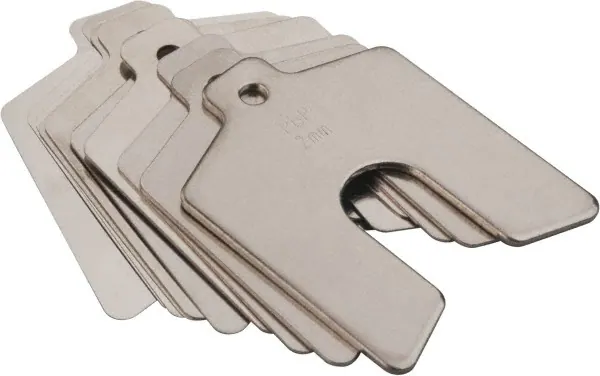
\includegraphics[scale=0.25]{Images/shims.png}
		\captionof{figure}{Shims of various thicknesses}
		\small\textsuperscript{Source: www.mscdirect.com/product/details/70475967}
		\label{fig:shims}
		
	\end{minipage}\hfill % these two lines must be close to each other
	\begin{minipage}{0.58\linewidth}
		
		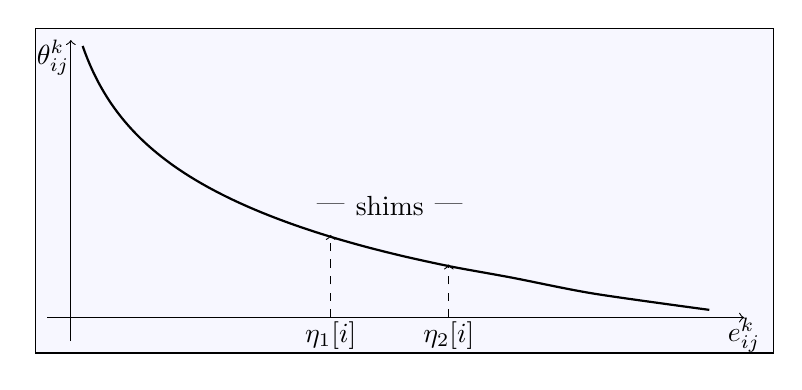
\begin{tikzpicture}[scale=0.75, samples=100]
			\filldraw[fill=blue!3!white, draw=black] (0, 0) rectangle (12.5, 5.5);
			\draw[->] (.2, .6) -- coordinate (x axis mid) (12, .6);
			\node at (5, 0.3) {$\eta_1[i]$};
			\node at (5, 2.5) {|};
			\node at (6, 2.5) {shims};
			\node at (7, 2.5) {|};
			\node at (7, 0.3) {$\eta_2[i]$};
			\node at (0.3, 5) {$\theta_{ij}^k$};
			\draw[->] (.6, .2) -- coordinate (y axis mid) (0.6, 5.3);
			\node at (12, 0.3) {$e_{ij}^k$};
			\draw[smooth, domain = 0.09:2, color=black, thick] plot (.3+1/\x,{4.2+log2(\x)});
			\draw[->, dashed] (5, 0.6)--(5, 2.0);
			\draw[->, dashed] (7, 0.6)--(7, 1.5);
		\end{tikzpicture}
		
		\captionof{figure}{$n_k$\/ edges $e_{ij}^k$\/ of $p_i$\/ sorted by $\theta_{ij}^k$\/ in non-ascending order}
		\label{fig:whip}		
	\end{minipage}
\end{table}


Figure \ref{fig:whip} represents the $n_k$\/ possible edges $e_{ij}^k$\/ of $p_i$\/ sorted by $\theta_{ij}^k$. \emph{mpShims}\/ starts with a greedy solution, stopping at the edge with index in $\eta_1[i]$ close to the local optimum (first phase). Then, considering even the edge with the index $\eta_2[i]$, it elaborates different possible complements for this pallet (second phase) and selects the best of these complements (third phase).


\begin{algorithm}[H]
	\caption{Solve a node with {\it mpShims}}  \label{alg:mpshims}
	\begin{algorithmic}[1]
		
		\Procedure{$SolveNode$}{$mpShims, k, G, numProcs,\ timeLim$}
		
		\State $G^* \gets G(V_k, E^Q_k)$ \label{best_so_far}
		
		\State Sort $M$ by $|p_i.d|$ in non-descending order \label{mpshims:pallets}
		
		\State $E^N_k \gets \{\}$ \label{mpshims:items}
		
		\State Let $E[1..m][1..n_k]$, where $E[i]$ is an array with $n_k$ edges $(p_i,t^k_j)$ sorted by $\theta_{ij}^k$ in non-ascending order, $1 \leq i \leq m$ \label{mpshims:edges}
		
		\State $limits \gets getLimits(0.75,\ 0.98,\ numProcs)$ \label{mpshims:limits}
		
		\State $shimsQueue \gets \{\}$ \label{mpshims:queue}
	
		\For{$lim \in limits$}
			\State $shimsSolve(G(V_k, E^Q_k),\ M,\ shimsQueue,\ lim,\ E)$ \label{mpshims:send}
		\EndFor
		
		\State $counter \gets |limits|$
		
		\While{$counter > 0$}
			
			\State $G \gets \varnothing$

			\While{$runtime < timeLim$} \Comment{Wait until there is a solution in the queue}
			
			\State $G \gets shimsQueue.Pop()$
				\If{$G \ne \varnothing$}
					\Break
				\EndIf
			\EndWhile
			
			\If{$f_s(G) > f_s(G^*)$}
				\State $G^* \gets G$ 
			\EndIf
			\State $counter \gets counter - 1$			
		
		\EndWhile		
		
		\Return $G^*(V_k, E^N_k \cup E^Q_k)$ \label{mpshims:return}
		
		\EndProcedure
	\end{algorithmic}
\end{algorithm}

Algorithm \ref{alg:mpshims} describes the {\it SolveNode} method when it receives {\it mpShims} as argument.

Line \ref{best_so_far} defines the best solution so far which is formed by a semi-loaded aircraft where pallets have been unloaded and some remain on board ($E^Q_k$) with consolidated items.

The Shims solution starts with the set of pallets closer to the center of gravity (\ref{mpshims:pallets}).

A new empty set of edges is created in line \ref{mpshims:items}.

Edges with items in node "k" to be loaded into not full pallets are defined in line \ref{mpshims:edges}.

Line \ref{mpshims:limits} creates a list of unique limits with values between 0.75 and 0.98, that will be sent to different parallel processes to generate diverse solutions.

A queue of shims solutions to be used by the child processes to send solution to the main process is defined in line \ref{mpshims:queue}.

The iteration in \ref{mpshims:send} publishes or triggers parallel processes to solve $G(V_k, E^Q_k)$.

In line \ref{mpshims:wait} the program hangs until each child process put a solution into the queue. Each solution is collected by the main process and compared with the best so far.

Finally, in line \ref{mpshims:return}, the best solution found is returned.


\begin{algorithm}[H]
	\caption{Shims solving method to be run in parallel}  \label{alg:shimsSolve}
	\begin{algorithmic}[1]
		
		\Procedure{$shimsSolve$}{$G,\ M,\ shimsQueue,\ limit,\ E$}
		
		\State $G(V_k,\ E^Q_k \cup E^N_k),\ \eta_1 \gets Greedy(k,\ G(V_k,\ E^Q_k),\ limit)$ \label{first_phase}
				
		\For{$i \gets 1$ to $m$}
	
			\State $\eta_2[i] \gets \eta_1[i]$	
			
			\State $volume \gets 0$	

			\Repeat \label{second_phase_begin}
				\State $\eta_2[i] \gets \eta_2[i] + 1$ 
				\State $e^k_{ij} \gets E[i][\eta_2[i]]$
				\State $volume \gets volume + t^k_j.v$
			\Until{($\eta_2[i] = n_k$) {\bf or} ($ volume \geq (2 - limit)*p_i.v)$)} \label{second_phase_end}
			
			\State $slack[i] \gets (1-limit) \times p_i.v$
			
			\State $E^N_k \gets E^N_k \cup getBestShims(i,\ \eta_1,\ \eta_2,\ E,\ k,\ slack[i])$ \label{third_phase}
		
		\EndFor
		
		\State $shimsQueue \gets shimsQueue \cup \{G(V_k, E^N_k \cup E^Q_k)\}$ \label{enqueue}
		
		\EndProcedure
		
	\end{algorithmic}
\end{algorithm}

Algorithm \ref{alg:shimsSolve}, line \ref{first_phase} corresponds to Shims' first phase. Lines  \ref{second_phase_begin}-\ref{second_phase_end} correspond to the Shims' second phase.
Line \ref{third_phase} corresponds to Shims' third phase. In the last line, \ref{enqueue}, {\it mpShims} puts the solution into the queue to be retrieved by the main process.


\begin{algorithm}[H]
	\caption{Get the best shims of edges that fills each pallet gap}  \label{alg:getBestShims}
	\begin{algorithmic}[1]
		
		\Procedure{$getBestShims$}{$i,\ \eta_1,\ \eta_2,\ E,\ k,\ slack$}
		
		\State $volume \gets 0$	
		
		\State $b \gets 1$
		\State $shims[b] \gets \{\}$  \label{empty_shims}
		\State $Set \gets Set \cup \{shims[b]\}$ \label{empty_set}
		
		\For{$x \gets \eta_1[i]$ to $\eta_2[i]$} \label{edges_indexes}
				

			\State $NewShims \gets$ {\bf True} \label{new_shims}
			\State $e_{ij}^k \gets E[i][x]$
			
			\For{$shims \in Set$} \label{shims_set}
							
				\If { $e_{ij}^k \not\in (E^N_k \cup shims)$ {\bf and} $e_{ij}^k$ is feasible  {\bf and}  $(t_j^k.v + volume) \leq slack[i]$}
				
					
					\State $shims \gets shims \cup \{e_{ij}^k\}$
					\State $volume \gets volume + t_j^k.v$
					\State $NewShims \gets$ {\bf False} \label{new_shims_false}
		
					\State {\bf break}
		
				\EndIf
			
			\EndFor 
		
			\If{$NewShims$} \label{new_shims2}
				\State $volume \gets 0$
				\State $b \gets b + 1$
				\State $shims[b] \gets \{\}$
				\State $shims[b] \gets shims[b] \cup \{e_{ij}^k\}$
				\State $Set \gets Set \cup \{shims[b]\}$
			\EndIf

		\EndFor 
		
		\State $sh_w \gets shims$, where $shims \in Set$ and $\sum_{e_{ab}^k \in shims} t_b^k.w$ is maximum  \label{best_weight}		
		\State $sh_v \gets shims$, where $shims \in Set$ and $\sum_{e_{ab}^k \in shims} t_b^k.v$ is maximum \label{best_volume}
		\State $sh_{best} \gets shims$, where $shims \in \{sh_w, sh_v\}$ and $\sum_{e_{ab}^k \in x} t_b^k.s$ is maximum \label{best_score}
		
		\Return $sh_{best}$
		
		\EndProcedure
		
	\end{algorithmic}
\end{algorithm}

Algorithm \ref{alg:getBestShims} describes the procedure do get the best Shims, the best subset of edges to fill each pallet gap. This algorithm follows the logic of the {\it First-Fit Decreasing} algorithm as described by \cite{JohnsonGarey1985}.

Line \ref{empty_shims} creates the first empty shims.
Line \ref{empty_set} creates the first set of shims from where the best shims will be chosen.

Line \ref{edges_indexes} iterate in the edges indexes range to find subsets of shims that fit into each pallet gap.

Initially, new shims creation is permitted (\ref{new_shims}), but it will only be created if the last edge could not be included in any shims from the set (\ref{new_shims2}). 

For each edge, iterate in all sets in a try to include it in any of the previous shims (\ref{shims_set}).
As the last edge was included, forbid a new shims creation (\ref{new_shims_false}).

Finally, select the best weight shims (\ref{best_weight}), the best volume shims (\ref{best_volume}), and the best score shims (\ref{best_score}) between these 2. The best score shims edges will be returned.

\section{Implementation and results}
\label{sec6}


As we are dealing with a new problem, which has been modeled by \cite{MesquitaSanches2023}, we use the same benchmarks of their work, which are based on the characteristics of real airlifts carried out by the {\em Brazilian Air Force}.
 
We test our methods with 126 different instances: six operational scenarios with 2 aircraft sizes and 3 to 7 nodes; and seven randomly generated item sets for three volume surpluses (1.2, 1.5, and 2.0 times aircraft volume capacities).


\subsection{Results obtained}


%The testing experiments are performed on a 64-bit, 16GiB, 3.2GHz, 8-core processor, 2 threads per core, AMD FX-8320E, with {\it Linux Ubuntu 22.04} as the operational system and {\it Python 3.10.4}\/ as the programming language.

The final experiments are performed on a 64-bit, 128GiB, 3.6GHz, 48-core processor, 2 threads per core, Intel Xeon, with {\it Linux CentOS 8} as the operational system and {\it Python 3.8.2} as the programming language.

For parallelization, we used the {\it Python Multi-processing} package, which implements {\it process-based parallelism} or {\it parallel shared memory algorithm}. According to \cite{Multi-processing}, {\it Multi-processing} is a package that supports spawning processes using an API similar to the {\it Python Threading} package.

According to \cite[p.271]{Breshears2009}, a {\it Process} is the operating system’s spawned and controlled entity that encapsulates an executing application. A process has two main jobs: the first is to hold the application's resources, and the second is to carry out the application's instructions. 

It is known that working concurrently opens up synchronization issues. But the {\it Multi-processing} package (mp) offers both local and remote concurrency, effectively side-stepping the global interpreter lock by using sub-processes instead of threads. Because of this, the {\it Multi-processing} module lets the programmer take full advantage of the fact that a machine has more than one processor, normally capable of 2 threads each.

By Amdahl's law, there is an optimal number of parallel executions for each problem in each environment. While working at IBM in 1967, Gene Amdahl developed the foundation for what became known as Amdahl's Law or Amdahl's Argument. Essentially, the law states that while a process can be decomposed into steps that may then be run in parallel, the time taken for the whole process will be significantly limited by the steps that remain serialized. So, we decided to run some tests to find the best number of parallel processes for each of this work's operational scenarios.

For each red bullet closest to the upper left corner, we call it {\it Utopia}, an impossible result with zero time duration and a possible best score. The blue bullets are experiments performed with the number of parallel processes indicated. The shortest distance from {\it Utopia} may reveal the most efficient parallel processes for the scenario (see Table \ref{tab:scenarios}). 


\begin{figure}[H]
	\begin{center}
		\begin{tikzpicture}[scale=0.8, samples=100]
			\begin{axis}[
				myplotstyle,
				xlabel={\bf mpShims computation times (s)},
				ylabel={\bf Score},
				]
				\addplot+[
				only marks,	
				nodes near coords = {\numProcs{}},
				visualization depends on = {value \thisrow{np} \as \numProcs},						
				]
				table[x=time, y=score, col sep=comma] {./csv/Shims_p1data20.csv};
			\end{axis}
			\fill [red] (canvas cs:x=0.1cm,y=5.6cm) circle (2pt);
		\end{tikzpicture}%
		~%
		%
		\begin{tikzpicture}[scale=0.8, samples=100]
		\begin{axis}[
			myplotstyle,
			xlabel={\bf mpACO computation times (s)},
			ylabel={\bf Score},
			]
			\addplot+[
			only marks,	
			nodes near coords = {\numProcs{}},
			visualization depends on = {value \thisrow{np} \as \numProcs},						
			]
			table[x=time, y=score, col sep=comma] {./csv/ACO_p1data20.csv};
		\end{axis}
		\fill [red] (canvas cs:x=0.1cm,y=5.6cm) circle (2pt);
	\end{tikzpicture}
		
	\end{center}
	\caption{ Scenario 1 performances with $1.2 \times volume$. }
	\label{fig:scenario1data20}
\end{figure}

Observing Figure \ref{fig:scenario1data20}, it may be noticed that the best number of processes for {\it Scenario 1} solved with {\it mpShims} (the closest to the {\it Utopia}) is \textbf{6}. Solved with {\it mpACO}, the best number is \textbf{8}. Table \ref{tab:numProcs} presents all methods, volumes percentages and scenarios numbers of best parallel processes to be run to solve all tours.

To build Table \ref{tab:numProcs}, it was necessary to determine the number of parallel processes that best solve each node. For this we created a procedure as in Algorithm \ref{alg:bestnum}.

\begin{algorithm}[H]
	\caption{Get the best number of parallel processes}  \label{alg:bestnum}
	\begin{algorithmic}[1]
		
		\Procedure{$getBestNPP$}{$scores,\ runtimes,\ procs$}
				
		\State $maxS   \gets max(scores)$
		\State $minS   \gets min(scores)$
		\State $maxR \gets max(runtimes)$
		\State $minR \gets min(runtimes)$
		
		\State $bestNPP \gets 0$, best number of parallel processes
		\State $minD \gets 999999999.9$		
		
		\For{$i \in |scores|$}
			\State $y = ( maxS - scores[i] )\ /\ (maxS   - minS  )$ \Comment{the Y axis leg}
			\State $x = ( runtimes[i] - minR )\ /\ (maxR - minR)$ \Comment{the X axis leg}
			\State $h = \sqrt{x^2 + y^2}$  \Comment{distance from {\it Utopia}}
			\If{$minD$ > $h$}
				\State $minD \gets h$
				\State $bestNPP \gets procs[i]$
			\EndIf
		
		\EndFor
		
		\Return $bestNPP$
		
		\EndProcedure
	\end{algorithmic}
\end{algorithm}


\vspace{2.0mm}

\begin{table}[H]
\centering
\caption{$bestNPP$ found for each scenario}  \label{tab:numProcs}
	\footnotesize
%\scriptsize
\begin{tabular}{rccccccc}
\toprule
                               &               &\multicolumn{6}{c}{\bf Scenarios} \\
                               \cmidrule{3-8}
{$method$}                     &{\it volume}&{\bf 1}&{\bf 2}&{\bf 3}&{\bf 4}&{\bf 5}&{\bf 6} \\
\toprule

\multirow{3}{*}{\it {mpShims}} &$1.2$& 6       & 4     & 4     & 4     & 2     & 2    \\ 
                               &$1.5$& 4       & 4     & 4     & 4     & 4     & 4    \\
                               &$2.0$& 4       & 4     & 4     & 2     & 2     & 4    \\
\midrule[.1pt]

\multirow{3}{*}{\it {mpACO}}   &$1.2$& 10      & 8     & 10    & 6     & 10    & 10   \\ 
                               &$1.5$& 10      & 6     & 12    & 8     & 10    & 8    \\
                               &$2.0$& 10      & 8     & 2     & 10    & 6     & 6    \\                               
\bottomrule		
\end{tabular}

\normalsize

\end{table}

Table \ref{tab:numProcs} presents the best numbers of parallel processes for each method, scenario, and volume surplus. As all numbers are less than or equal to 12, any hand-held computer with 8 cores can yield efficient solutions, as normally each core may be capable of 2 threads.

To find these values we submitted to test 1, 2, 4, 6, 8, 10, 12, 14, 16 parallel processes.


\vspace{2.0mm}

\begin{table}[H]
	\centering
	\caption{Volume surpluses, methods and scenarios results}  \label{tab:results}
	\footnotesize
	%\scriptsize
	\begin{tabular}{cccccccccc}
		\toprule
		              &            &                  &\multicolumn{6}{c}{\bf Scenarios}              &{\bf Normalized}\\
		\cmidrule{4-9}		
		{\bf Surplus} & {$method$} &{\bf Results}     &{\bf 1}&{\bf 2}&{\bf 3}&{\bf 4}&{\bf 5}&{\bf 6}&{\bf Speed-up} \\
		\toprule


		
		\multirow{6}{*}{$1.2$} &\multirow{2}{*}{ $mpShims^{0.7s}$}& $f$                & 5.70  & 3.09  & 2.94  & 2.90  & 2.79  & 5.70  & 0.91  \\%2312
		                       &                                 & {\bf run-time (s)} & 1     & 3     & 7     & 26    & 97    & 267   & 70  \\%390
		                       \cmidrule{2-10}
		                       &\multirow{2}{*}{ $mpACO^{60s}$}   & $f$                & 6.42  & 3.78  &  3.19 & 3.17  & 2.97  & 5.87  & 1.00  \\ %2540
                               &                                 & {\bf run-time (s)} & 16    & 282   &  314  & 1334  & 6945  & 18883 & 1  \\ %27162
		\cmidrule{2-10}		                       
							   &\multirow{2}{*}{ $mpACO^{0.7s}$}  & $f$                &&&&&&&\\
							   &                                 & {\bf run-time (s)} &&&&&&&\\                               
		\midrule
		\multirow{6}{*}{$1.5$} &\multirow{2}{*}{ $mpShims^{0.7s}$}& $f$                & 8.15  & 4.22  & 4.40  & 4.01  & 3.51  & 7.08  &   \\
		                       &                                 & {\bf run-time (s)} & 1     & 5     & 12    & 45    & 244   & 737   &   \\
		\cmidrule{2-10}
		                       &\multirow{2}{*}{ $mpACO^{60s}$}   & $f$                & 9.50  & 5.01  & 4.60  & 4.28  &&&\\
		                       &                                 & {\bf run-time (s)} & 9     & 344   & 787   & 1525  &&&\\
		\cmidrule{2-10}		                       
							   &\multirow{2}{*}{ $mpACO^{0.7s}$}  & $f$                &&&&&&&\\
							   &                                 & {\bf run-time (s)} &&&&&&&\\		                       
		\midrule
		\multirow{6}{*}{$2.0$} &\multirow{2}{*}{ $mpShims^{0.7s}$}& $f$                & 11.31 & 6.29  & 5.54  & 5.83  & 5.05  & 10.63 &   \\
		                       &                                 & {\bf run-time (s)} & 2     & 14    & 34    & 106   & 477   & 2417  &   \\
		\cmidrule{2-10}
		                       &\multirow{2}{*}{ $mpACO^{60s}$}   & $f$                &&&&&&&\\
		                       &                                 & {\bf run-time (s)} &&&&&&&\\
		\cmidrule{2-10}		                       
		                       &\multirow{2}{*}{ $mpACO^{0.7s}$}  & $f$                &&&&&&&\\
							   &                                 & {\bf run-time (s)} &&&&&&&\\
		\bottomrule	
		

	\end{tabular}
\textsuperscript{The numbers 0.7s and 60s as superscript on the methods names represent the time limit per node.}	
\normalsize
\end{table}


\section{Conclusions}
\label{sec7}

xxxxx

\section*{Acknowledgments}

This research was partially supported by \textit{São Paulo Research Foundation} (FAPESP, grant 2016/01860-1).

%\bibliographystyle{elsarticle-num} % descomentar antes de submeter
\bibliographystyle{elsarticle-harv} % comentar antes de submeter

%\section*{References}

\bibliography{references}

\end{document}
